\documentclass[11pt]{article}
\usepackage{amssymb}
\usepackage{amsthm}
\usepackage{enumitem}
\usepackage{amsmath, physics}
\usepackage{bm}
\usepackage{adjustbox}
\usepackage{mathrsfs}
\usepackage{graphicx}
\usepackage{siunitx}
\usepackage[mathscr]{euscript}

\title{\textbf{Solved selected problems of Modern Physics for Scientists and Engineers - John Taylor}}
\author{Franco Zacco}
\date{}

\addtolength{\topmargin}{-3cm}
\addtolength{\textheight}{3cm}

\newcommand{\N}{\mathbb{N}}
\newcommand{\Z}{\mathbb{Z}}
\newcommand{\Q}{\mathbb{Q}}
\newcommand{\R}{\mathbb{R}}
\newcommand{\diam}{\text{diam}}
\newcommand{\cl}{\text{cl}}
\newcommand{\bdry}{\text{bdry}}
\newcommand{\inter}{\text{int}}
\newcommand{\hatx}{\bm{\hat{x}}}
\newcommand{\haty}{\bm{\hat{y}}}
\newcommand{\hatz}{\bm{\hat{z}}}
\newcommand{\hatrho}{\bm{\hat{\rho}}}
\newcommand{\hatphi}{\bm{\hat{\phi}}}
\newcommand{\hatr}{\bm{\hat{r}}}
\newcommand{\hattheta}{\bm{\hat{\theta}}}
\newcommand{\sci}[1]{\times 10^{#1}}

\theoremstyle{definition}
\newtheorem*{solution*}{Solution}
\renewcommand*{\proofname}{\bf{Solution}}

\begin{document}
\maketitle
\thispagestyle{empty}

\section*{Chapter 7 - The Schrödinger Equation in One Dimension}

\begin{proof}{\textbf{7.8}}
    Equation (7.118) states that
    \begin{align*}
        y(x,t) = A\sin kx\cos\omega t
    \end{align*}
    We know that $k = 2\pi/\lambda$ and $\omega = 2\pi/T$ hence the equation
    becomes
    \begin{align*}
        y(x,t) = A\sin \frac{2\pi x}{\lambda}\cos \frac{2\pi t}{T}
    \end{align*}
    Let us take a point $x = x_0 + \lambda$ with $t$ fixed then
    \begin{align*}
        y(x_0 + \lambda,t)
        &= A\sin \left(\frac{2\pi (x_0 + \lambda)}{\lambda}\right)
        \cos \frac{2\pi t}{T}\\
        &=  A\sin \left(\frac{2\pi x_0}{\lambda} + 2\pi\right)
        \cos \frac{2\pi t}{T}\\
        &=  A\bigg[\sin \frac{2\pi x_0}{\lambda}\cos 2\pi
        + \cos \frac{2\pi x_0}{\lambda}\sin 2\pi \bigg]
        \cos \frac{2\pi t}{T}\\
        &=  A\bigg[\sin \frac{2\pi x_0}{\lambda} + 0 \bigg]
        \cos \frac{2\pi t}{T}\\
        &=  A\sin \frac{2\pi x_0}{\lambda}\cos \frac{2\pi t}{T}\\
        &= y(x_0,t)
    \end{align*}
    Where we used the trigonometric identity
    $\sin(\alpha + \beta) = \sin\alpha\cos\beta + \cos\alpha\sin\beta$.
    This shows that the wave has the same value if we move from $x_0$
    to a point $x_0 + \lambda$.

    In the same way, let us take $t = t_0 + T$ with $x$ fixed then
    \begin{align*}
        y(x, t_0 + T)
        &= A\sin \frac{2\pi x}{\lambda}
        \cos \left(\frac{2\pi (t_0 + T)}{T}\right)\\
        &= A\sin \frac{2\pi x}{\lambda}
        \cos \left(\frac{2\pi t_0}{T} + 2\pi\right)\\
        &= A\sin \frac{2\pi x}{\lambda}
        \bigg[\cos\frac{2\pi t_0}{T}\cos 2\pi - \sin\frac{2\pi t_0}{T}\sin 2\pi\bigg]\\
        &= A\sin \frac{2\pi x}{\lambda}\bigg[\cos\frac{2\pi t_0}{T} - 0\bigg]\\
        &= A\sin \frac{2\pi x}{\lambda}\cos\frac{2\pi t_0}{T}\\
        &= y(x, t_0)
    \end{align*}
    Where we used the trigonometric identity
    $\cos(\alpha + \beta) = \cos\alpha\cos\beta - \sin\alpha\sin\beta$.
\end{proof}
\cleardoublepage
\begin{proof}{\textbf{7.9}}
\begin{itemize}
    \item [\textbf{(a)}] For $t = 0.05~s$ we have that
    \begin{center}
        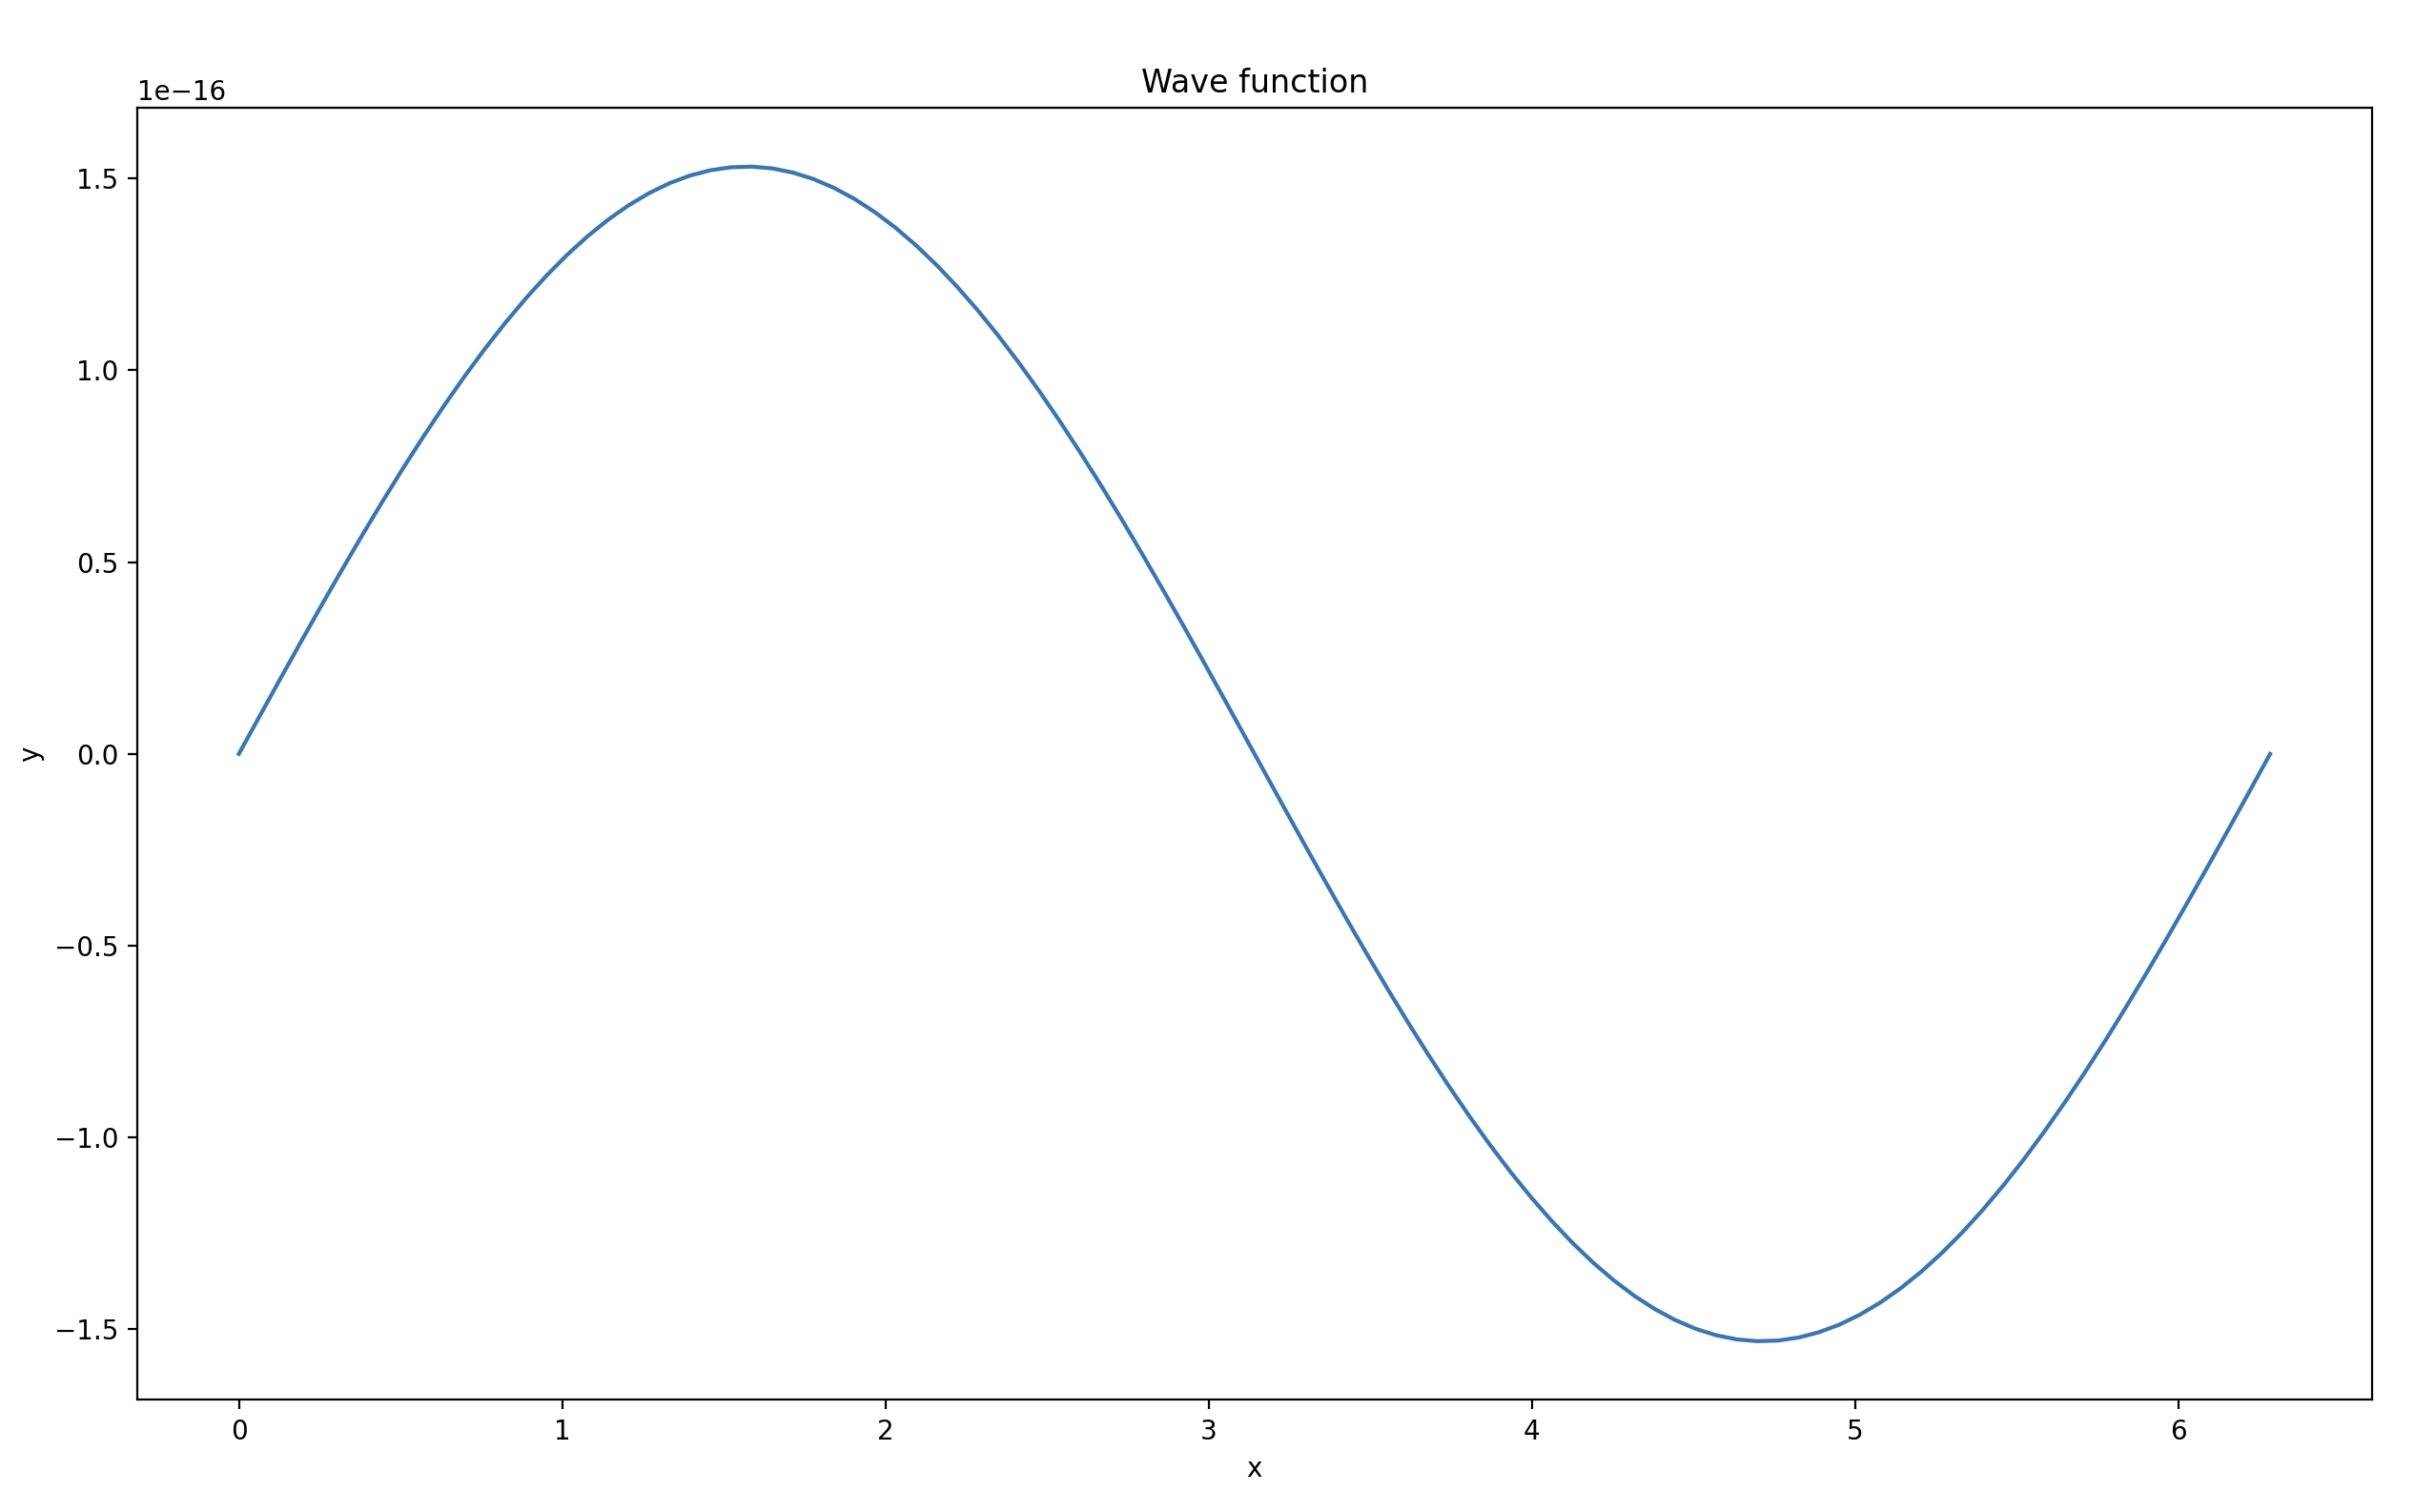
\includegraphics[scale=0.25]{ch7-7.9-1.png}
    \end{center}
    And for $t = 0.1~s$ we get that
    \begin{center}
        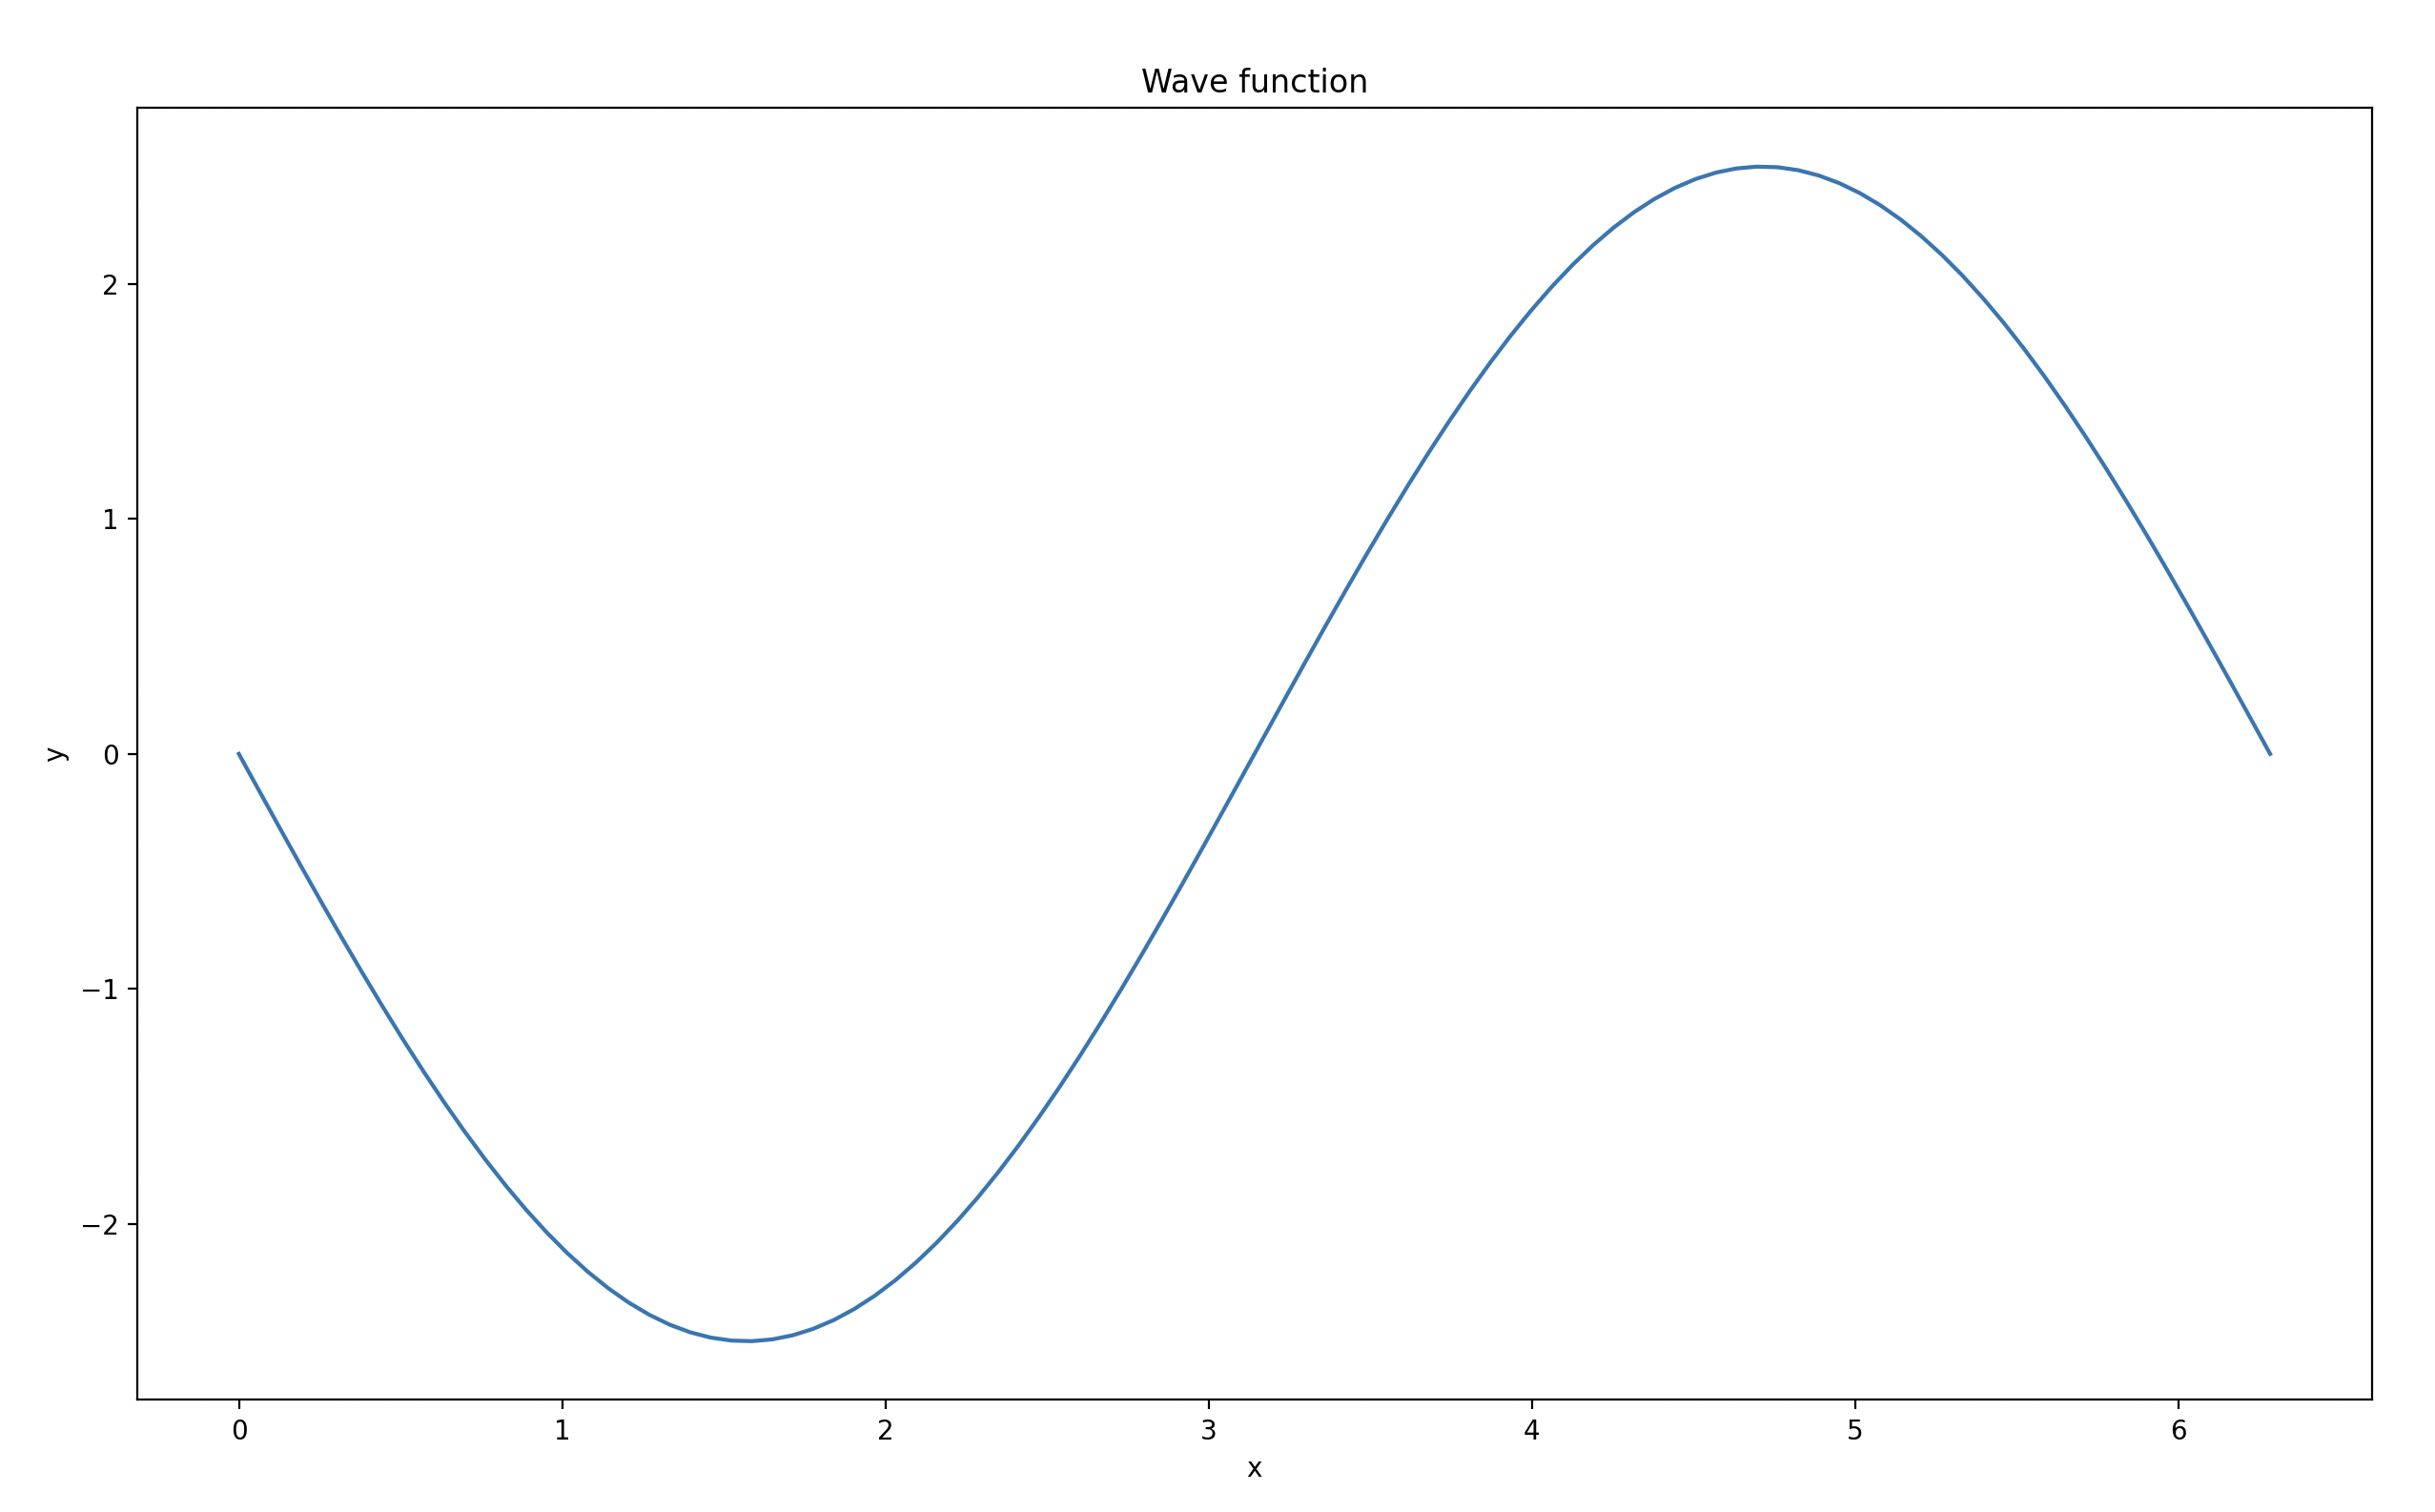
\includegraphics[scale=0.25]{ch7-7.9-2.png}
    \end{center}
\cleardoublepage
    \item [\textbf{(b)}] Let $x$ be fixed then the derivative of (7.118) with
    respect to $t$ gives us
    \begin{align*}
        \pdv{y(x,t)}{t} = -\omega A\sin kx\sin\omega t
    \end{align*}
    Then for $t = 0.05~s$ the transverse velocity is
    \begin{center}
        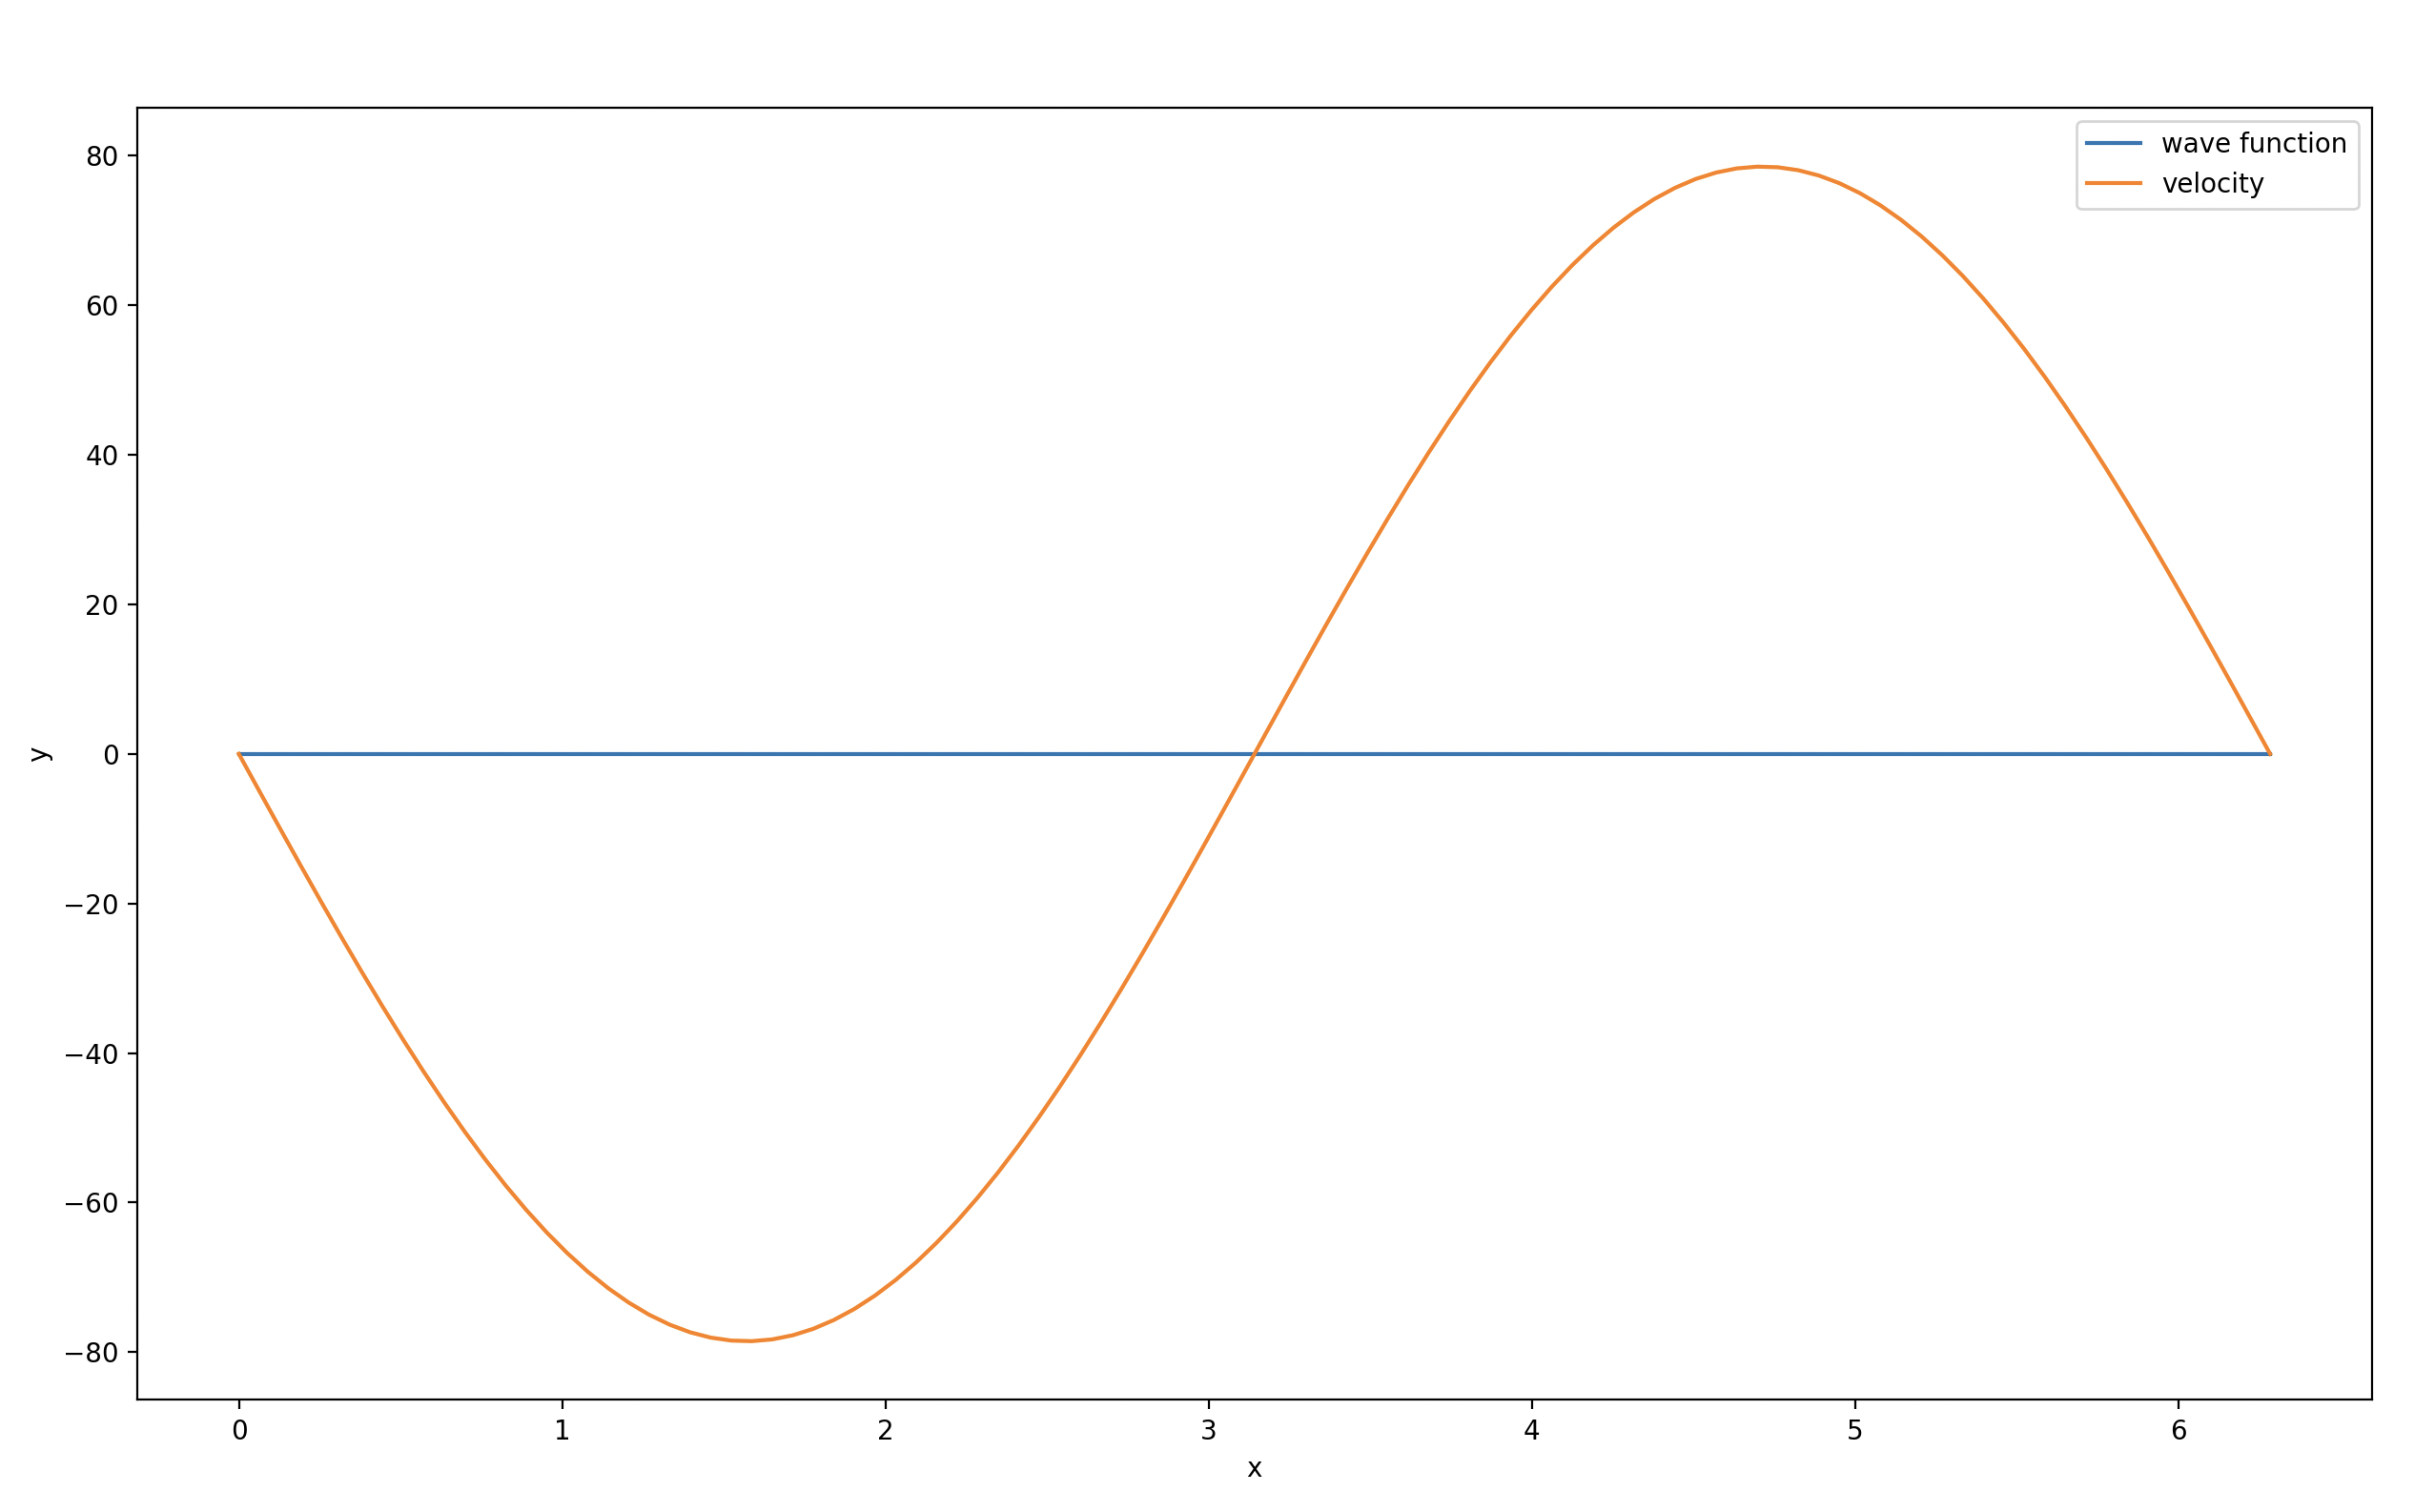
\includegraphics[scale=0.25]{ch7-7.9-3.png}
    \end{center}
    So the velocity is high when the wave function amplitude is small.

    Finally, for $t = 0.1~s$ we get that
    \begin{center}
        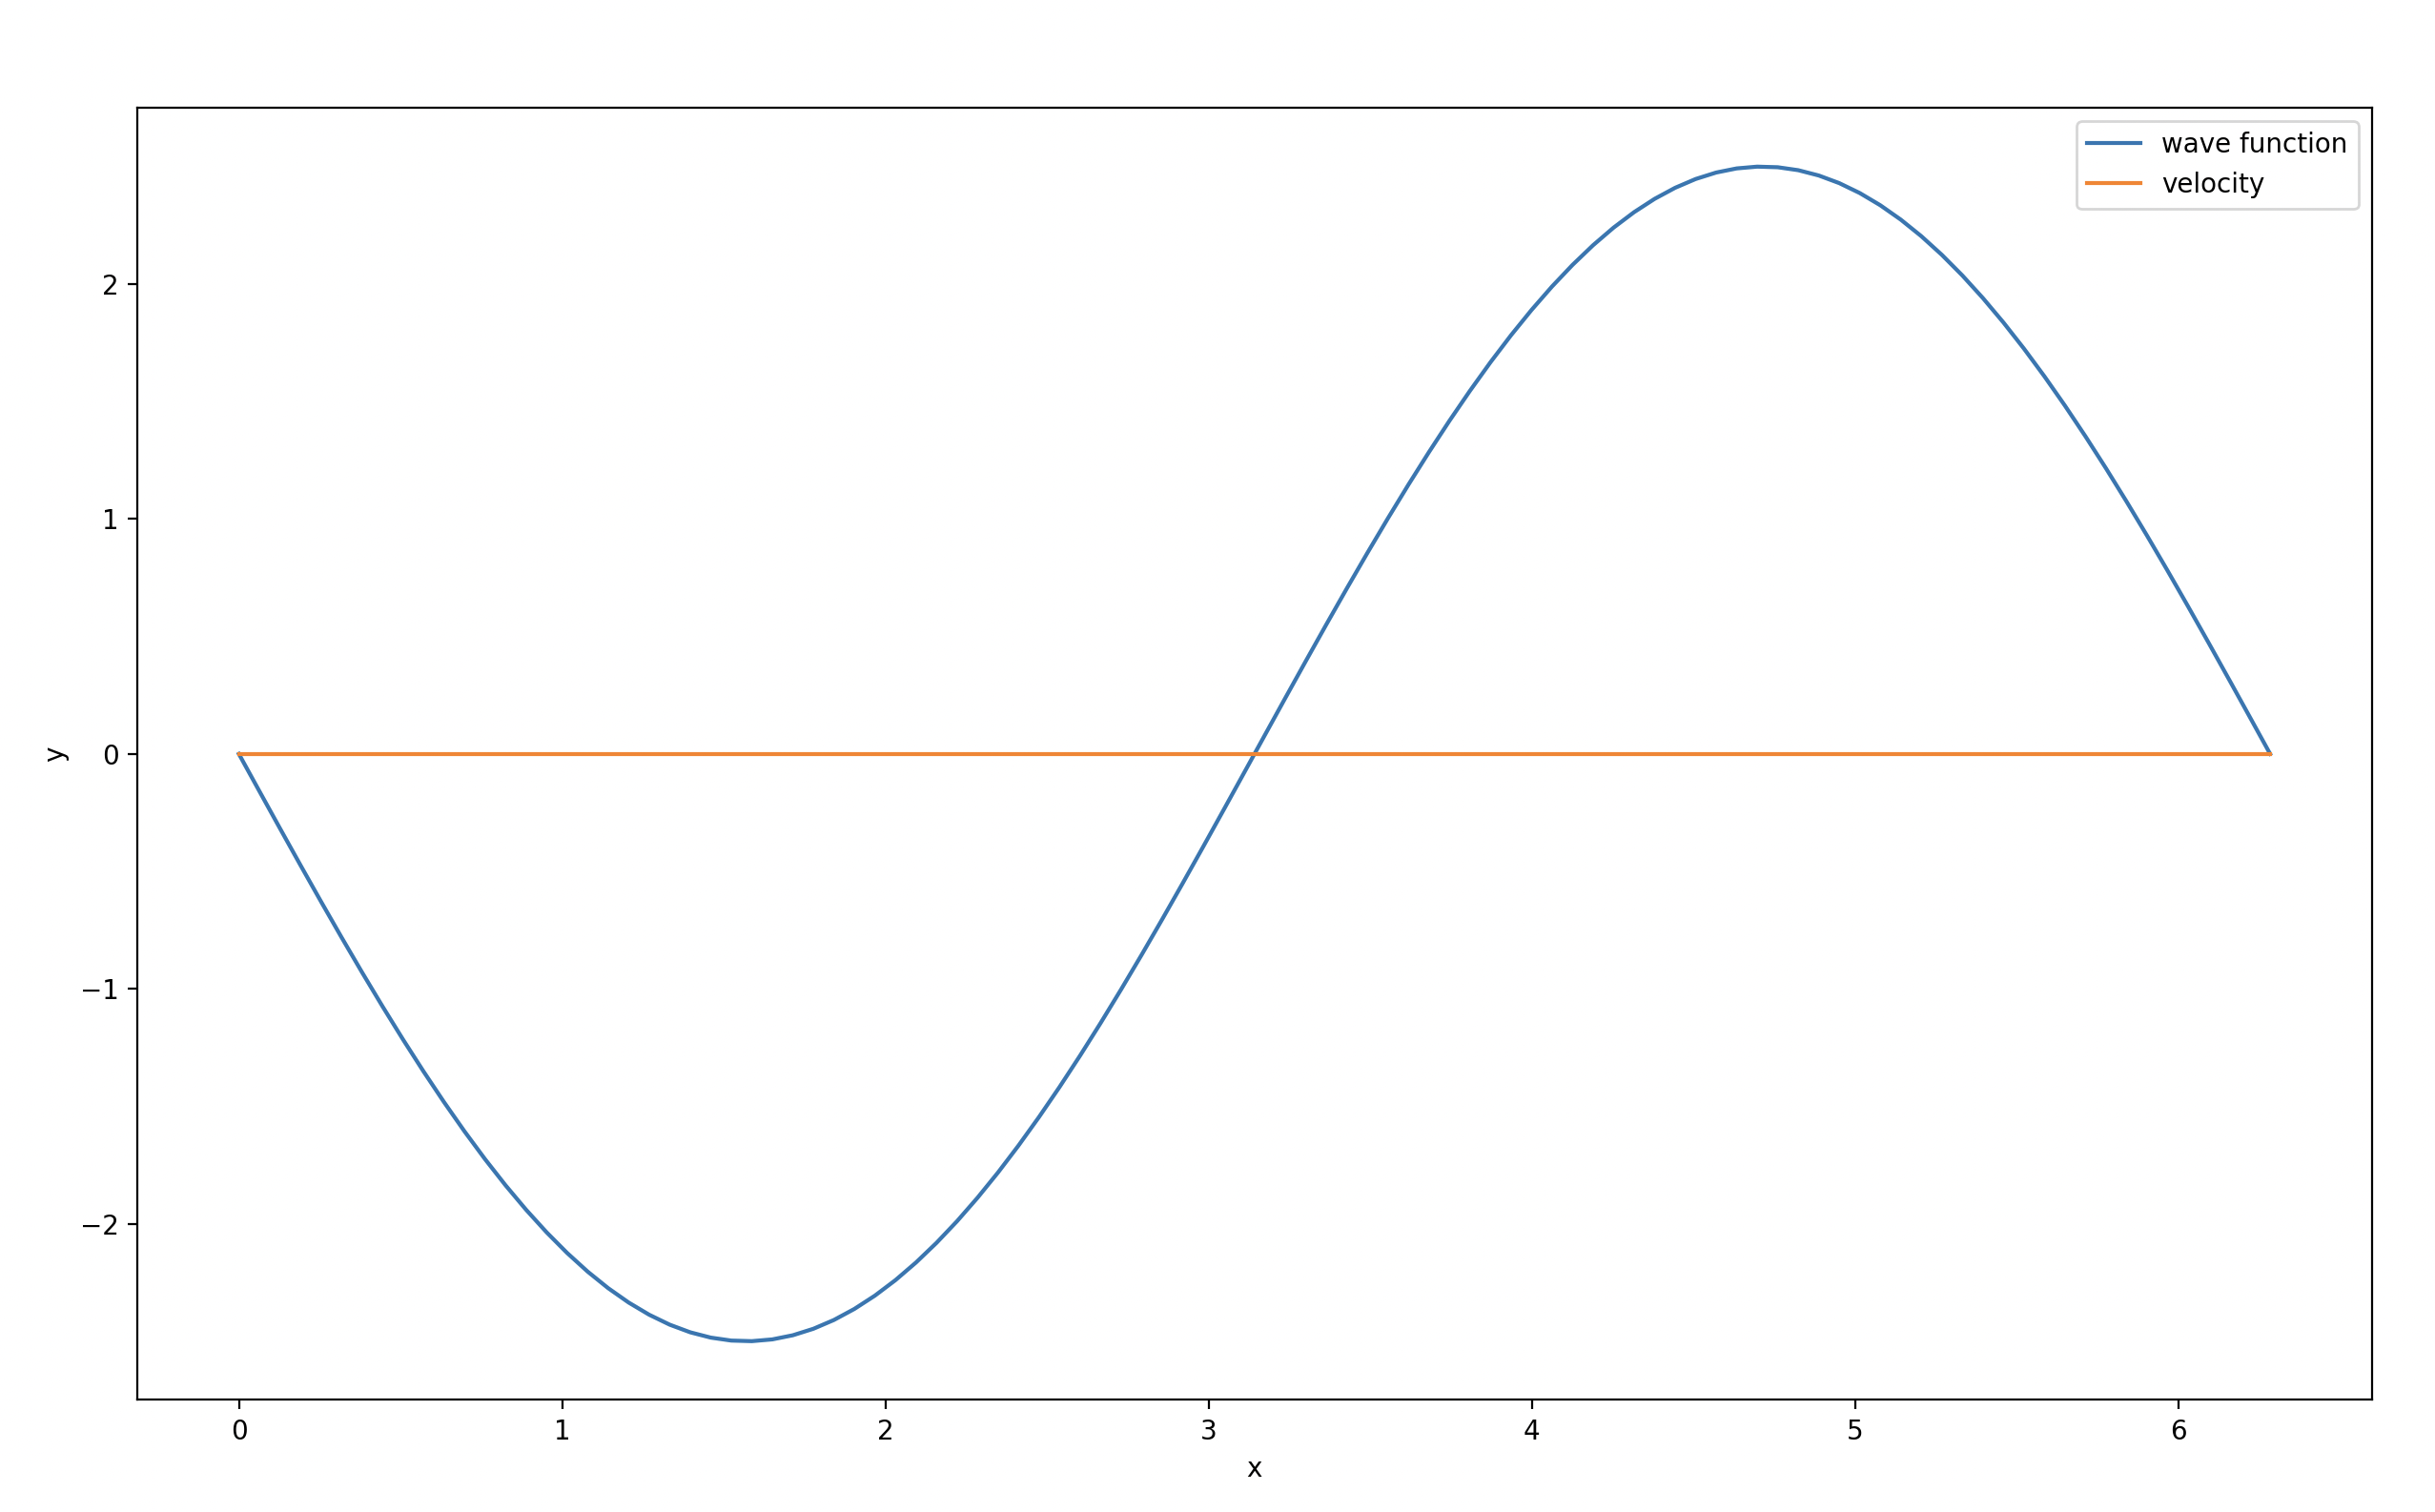
\includegraphics[scale=0.25]{ch7-7.9-4.png}
    \end{center}
    Here the velocity is small when the wave function amplitude if significant.
\end{itemize}
\end{proof}
\cleardoublepage
\begin{proof}{\textbf{7.11}}
\begin{itemize}
    \item [\textbf{(a)}] Let $z = x + iy$ then
    \begin{align*}
        |z|^2 = x^2 + y^2 = x^2 + y^2 + ixy - ixy = (x + iy)(x - iy) =zz^*
    \end{align*}
    \item [\textbf{(b)}] Let now $w = u + iv$ then
    \begin{align*}
        |zw| &= |(x + iy)(u + iv)|\\
        &= |xu +ixv +iuy - vy|\\
        &= |(xu - vy) + i(xv + uy)|\\
        &= \sqrt{(xu - vy)^2 + (xv + uy)^2}\\
        &= \sqrt{(xu)^2 - 2xuvy + (vy)^2 + (xv)^2 + 2xuvy + (uy)^2}\\
        &= \sqrt{(xu)^2 + (vy)^2 + (xv)^2 + (uy)^2}\\
        &= \sqrt{u^2(x^2 + y^2) + v^2(x^2 + y^2)}\\
        &= \sqrt{(x^2 + y^2)(u^2 + v^2)}\\
        &= |z||w|
    \end{align*}
    \item [\textbf{(c)}] Let's compute $|\Psi(x,t)|$ as follows
    \begin{align*}
        |\Psi(x,t)| = |\psi(x)e^{-i\omega t}| = |\psi(x)||e^{-i\omega t}|
        = |\psi(x)|
    \end{align*}
    Where we used that $|e^{-i\omega t}| = 1$.
\end{itemize}
\end{proof}

\cleardoublepage
\begin{proof}{\textbf{7.17}}
The lowest energy for an electron in a one-dimensional box is given by
\begin{align*}
    E_1 &= \frac{\pi^2\hbar^2}{2ma^2}\\
    &= \frac{\pi^2\cdot (6.582 \times 10^{-16}~eVs)^2}
    {2\cdot 510.99 \times 10^3~eV/c^2 \cdot (0.2\times 10^{-9}~m)^2}\\
    &= 1.04595 \times 10^{-16}~eV c^2 s^2/m^2\\
    &= 9.40105~eV
\end{align*}
So the next two lowest energies are
\begin{align*}
    E_2 &= 2^2 E_1 = 37.6042~eV\\
    E_3 &= 3^2 E_1 = 84.60945~eV
\end{align*}
\end{proof}
\begin{proof}{\textbf{7.18}}
The lowest energy of a proton in a one-dimensional box is given by
\begin{align*}
    E_1 &= \frac{\pi^2\hbar^2}{2ma^2}\\
    &= \frac{\pi^2\cdot (6.582 \times 10^{-16}~eVs)^2}
    {2\cdot 938.27\times 10^{6}~eV/c^2 \cdot (5\times 10^{-15}~m)^2}\\
    &= 9.11418\times 10^{-11}~eV c^2 s^2/m^2\\
    &= 8.1918~MeV
\end{align*}
So the next two lowest energies are
\begin{align*}
    E_2 &= 2^2 E_1 = 32.7672~MeV\\
    E_3 &= 3^2 E_1 = 73.7262~MeV
\end{align*}
\end{proof}

\cleardoublepage
\begin{proof}{\textbf{7.21}}
    Let $\Delta p = \hbar k$ and $\Delta x = a/2$ so using that $k = n\pi/a$
    we get that
    \begin{align*}
        \Delta x \Delta p = \frac{\hbar k a}{2} = n\pi\frac{\hbar}{2}
    \end{align*}
    Therefore we see that
    $\Delta x \Delta p = n\pi\frac{\hbar}{2}> \frac{\hbar}{2}$ so these
    uncertainties are consistent with the Heisenberg uncertainty principle.
\end{proof}
\begin{proof}{\textbf{7.23}}
The coefficients $A$ and $B$ in the wave function for a negative-energy state
in the rigid box needs to satisfy $A + B = 0$ hence $A = -B$ but also 
must satisfy $Ae^{\alpha a} + Be^{-\alpha a} = 0$ hence replacing we have that
\begin{align*}
    -Be^{\alpha a} + Be^{-\alpha a} &= 0\\
    B(e^{-\alpha a} - e^{\alpha a}) &= 0\\
    B &= 0
\end{align*}
And since $A = -B$ then $A = 0$.
\end{proof}

\cleardoublepage
\begin{proof}{\textbf{7.30}}
\begin{itemize}
\item [\textbf{(a)}] The probability distribution for the second excited state
$n = 3$ of a particle in a rigid box of length $a$ is 
\begin{align*}
    |\psi(x)|^2 = \frac{2}{a}\sin^2\bigg(\frac{3\pi x}{a}\bigg)
\end{align*}
We sketch it below
\begin{center}
    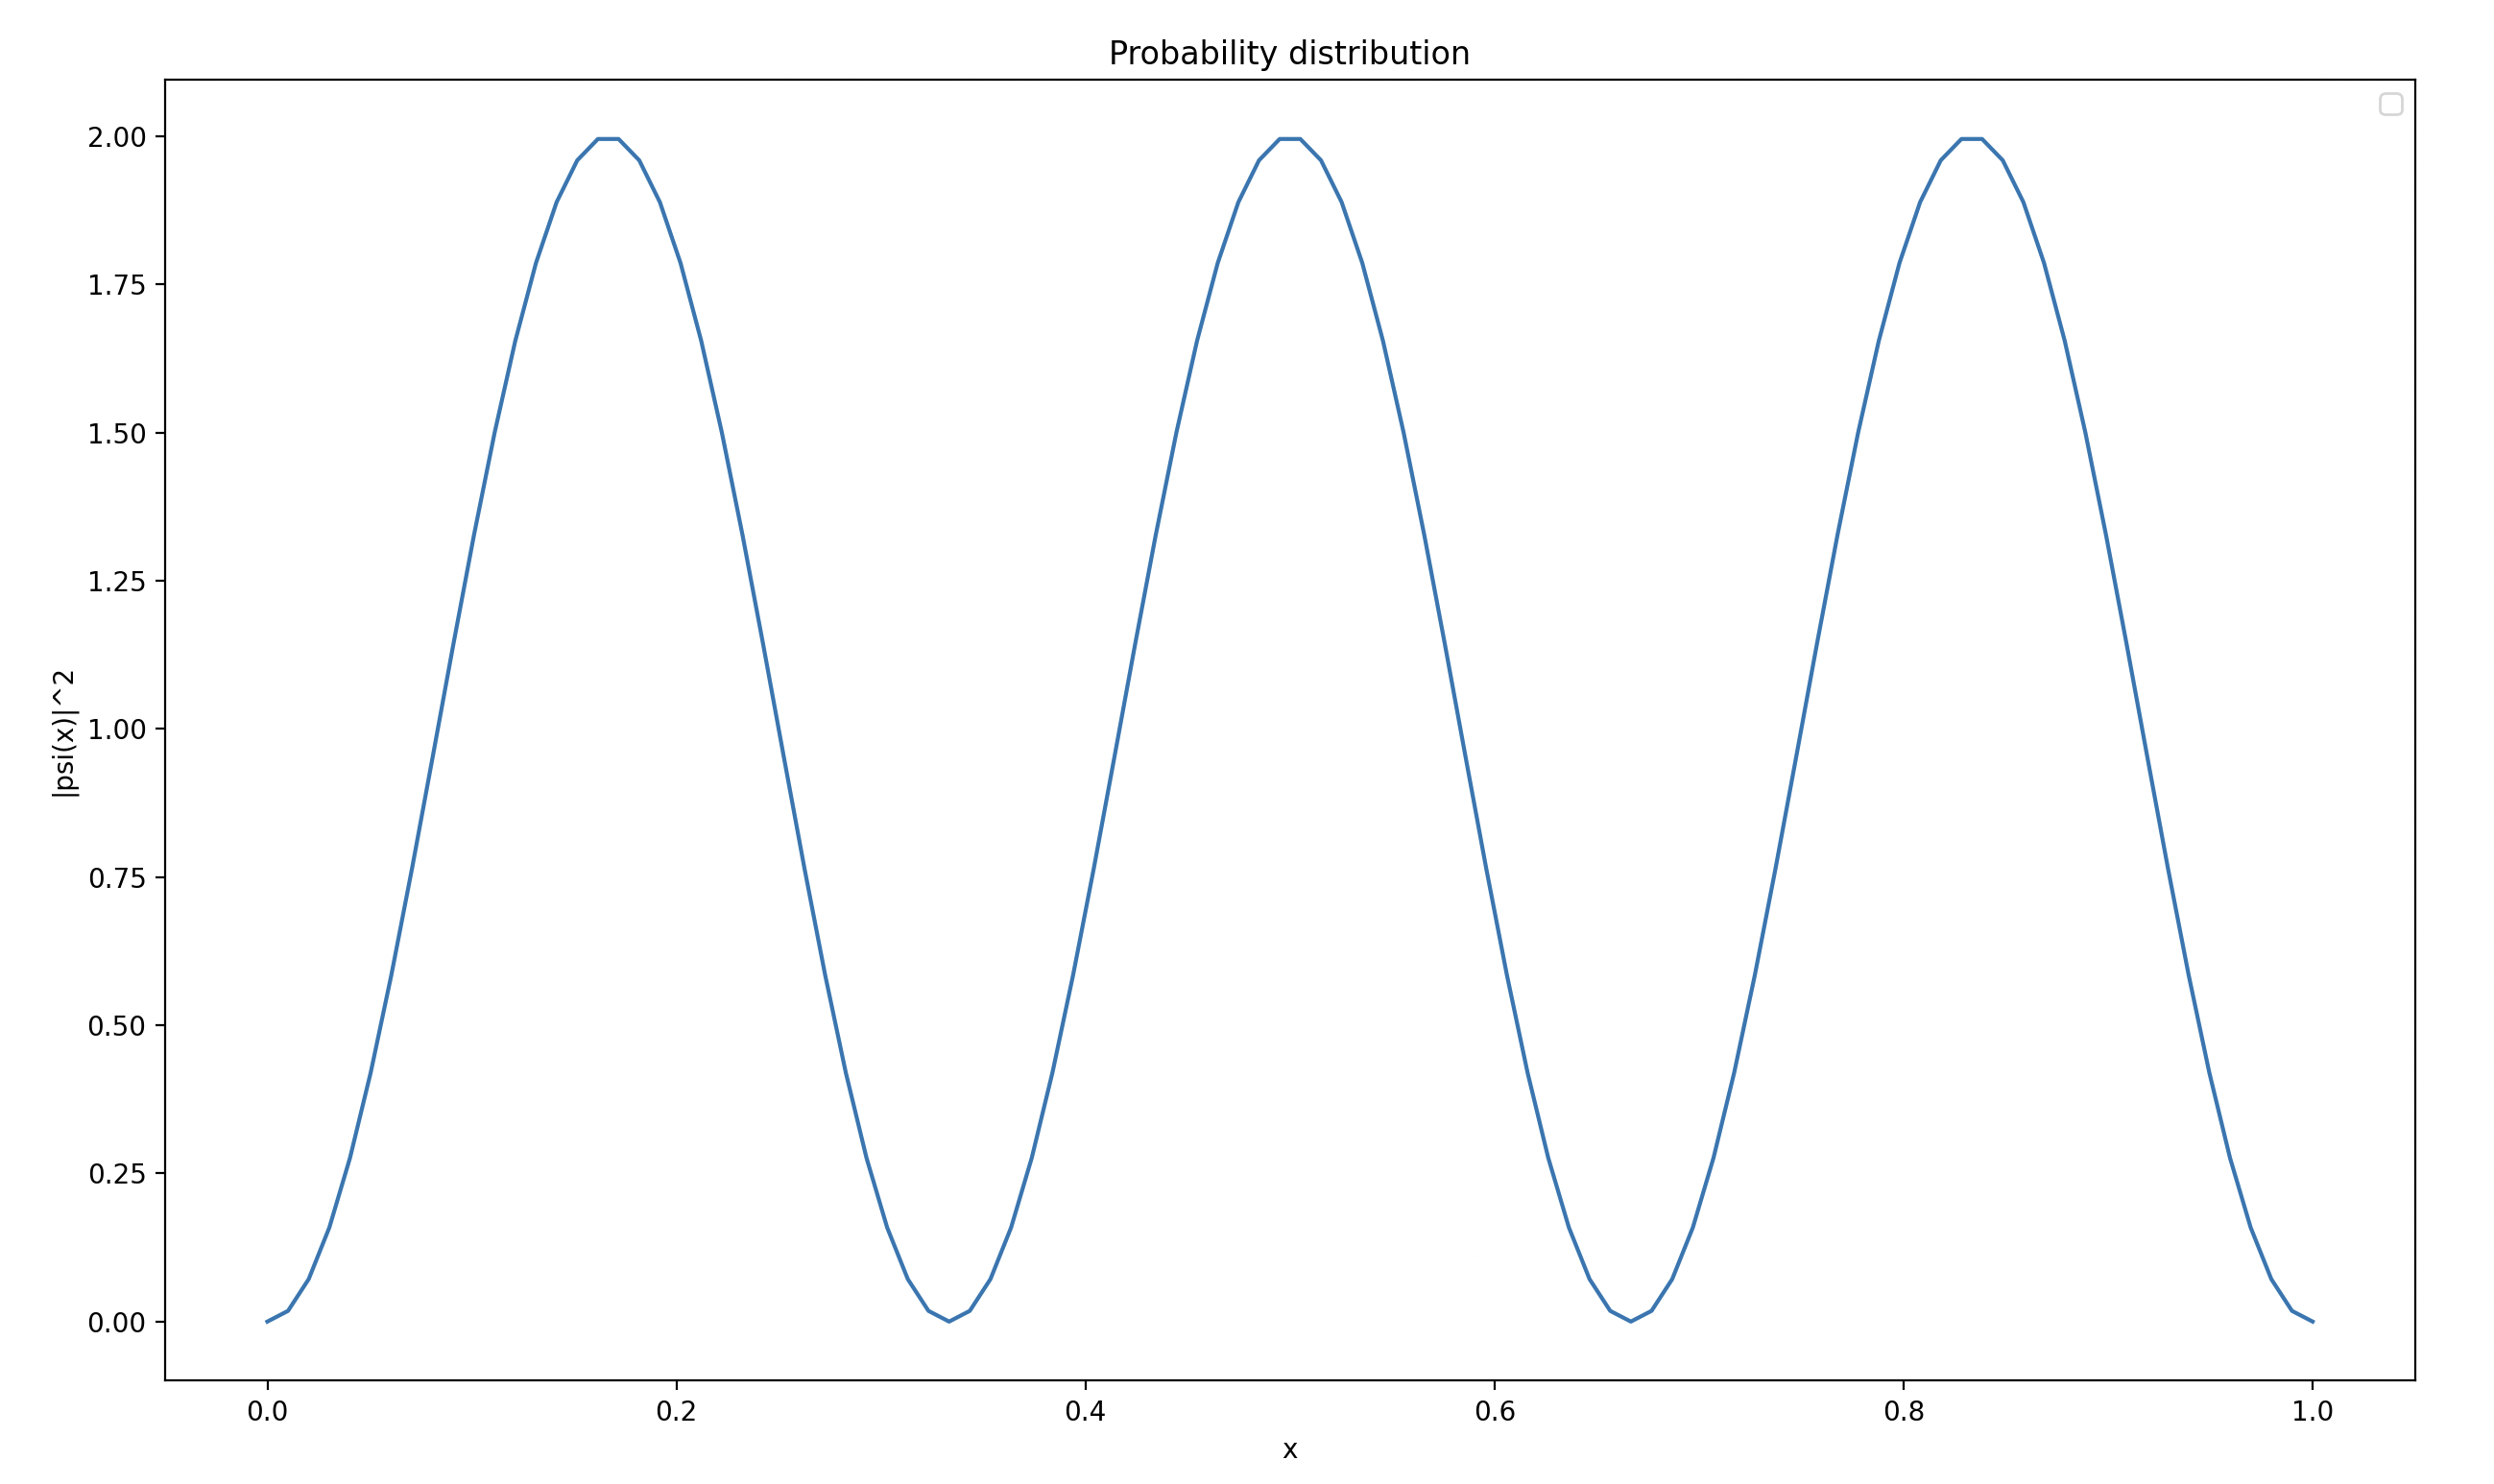
\includegraphics[scale=0.28]{ch7-7.30.png}
\end{center}
\item [\textbf{(b)}] The most probable values $x_{mp}$ are the values of $x$ for
which $|\psi(x)|^2$ is maximum, we see that this happens for 
$$x_{mp} \in \bigg\{\frac{a}{6}, \frac{a}{2}, \frac{5a}{6}\bigg\}$$
\item [\textbf{(c)}] The probability of finding the particle in the interval
$[0.5a, 0.51a]$ is
\begin{align*}
    P(0.5a \leq x \leq 0.51a) \approx |\psi(0.5a)|^2 \Delta x
    = \frac{2}{a}\sin^2\bigg(\frac{3\pi}{2}\bigg) \cdot 0.01a = 0.02 = 2~\%
\end{align*}
And the probability of finding the particle in the interval $[0.75a, 0.76a]$ is
\begin{align*}
    P(0.75a \leq x \leq 0.76a) \approx |\psi(0.75a)|^2 \Delta x
    = \frac{2}{a}\sin^2\bigg(\frac{9\pi}{4}\bigg) \cdot 0.01a = 0.001 = 0.1~\%
\end{align*}
\end{itemize}
\end{proof}

\cleardoublepage
\begin{proof}{\textbf{7.32}}
    The probability of finding a particle in the ground state of a rigid box
    between $x=0$ and $x=a/3$ is given by
    \begin{align*}
        P(0 \leq x \leq a/3)
        &= \int_{0}^{a/3} |\psi(x)|^2~dx\\
        &= \frac{2}{a}\int_{0}^{a/3} \sin^2\bigg(\frac{\pi x}{a}\bigg)~dx\\
        &= \frac{1}{a}\int_{0}^{a/3}
        \bigg[1 - \cos\bigg(\frac{2\pi x}{a}\bigg)\bigg]~dx\\
        &= \frac{1}{a}\bigg[
        x - \frac{a}{2\pi}\sin\bigg(\frac{2\pi x}{a}\bigg)\bigg]_{0}^{a/3}\\
        &= \frac{1}{a}\bigg[
        \frac{a}{3} - \frac{a}{2\pi}\sin\bigg(\frac{2\pi}{3}\bigg) - 0\bigg]\\
        &= \frac{1}{3} - \frac{\sqrt{3}}{4\pi}\\
        &= 0.1955
    \end{align*}
\end{proof}

\cleardoublepage
\begin{proof}{\textbf{7.34}}
The probability distribution for the second excited state
$n = 3$ of a particle in a rigid box of length $a$ is 
\begin{align*}
    |\psi(x)|^2 = \frac{2}{a}\sin^2\bigg(\frac{3\pi x}{a}\bigg)
\end{align*}
Hence the integral becomes
\begin{align*}
    \langle x\rangle &= \int_{0}^a x|\psi(x)|^2~dx\\
    &= \frac{2}{a}\int_{0}^a x\sin^2\bigg(\frac{3\pi x}{a}\bigg)~dx\\
    &= \frac{1}{a}\int_{0}^a x\bigg(1 - \cos(\frac{6\pi x}{a})\bigg)~dx\\
    &= \frac{1}{a}\left[\int_{0}^a x~dx - \int_{0}^a x\cos(\frac{6\pi x}{a})dx\right]
\end{align*}
Then taking $u = x$ and $dv = \cos(6\pi x/a) dx$ we get that
$du = dx$ and $v = \int \cos(6\pi x/a) dx = a\sin(6\pi x/a)/6\pi$ hence
\begin{align*}
    \langle x\rangle &= \frac{1}{a}\left[\frac{a^2}{2} 
    - \int_{0}^a x\cos(\frac{6\pi x}{a})dx\right]\\
    &= \frac{a}{2}
    - \frac{1}{a}\left[\frac{ax\sin(6\pi x/a)}{6\pi}\bigg|_0^a
    - \int_{0}^a \frac{a\sin(6\pi x/a)}{6\pi} dx\right]\\
    &= \frac{a}{2} - 0 + \frac{1}{6\pi}\int_{0}^a \sin(6\pi x/a) dx\\
    &= \frac{a}{2}
\end{align*}
\end{proof}

\cleardoublepage
\begin{proof}{\textbf{7.35}}
\begin{itemize}
\item [\textbf{(a)}] Let us evaluate the integral (7.122) for a particle in the
ground state in a rigid box of length $a$ from $x=0$ to $x=c$ where $c \leq a$
\begin{align*}
    P(0 \leq x \leq c) &= \int_0^c |\phi(x)|^2~dx\\
    &= \frac{2}{a} \int_0^c \sin^2\bigg(\frac{\pi x}{a}\bigg)~dx\\
    &= \frac{1}{a}\bigg[
    x - \frac{a}{2\pi}\sin\bigg(\frac{2\pi x}{a}\bigg)\bigg]_{0}^{c}\\
    &= \frac{1}{a}\bigg[
    c - \frac{a}{2\pi}\sin\bigg(\frac{2\pi c}{a}\bigg) - 0\bigg]\\
    &= \frac{c}{a} - \frac{1}{2\pi}\sin\bigg(\frac{2\pi c}{a}\bigg)
\end{align*}
\item [\textbf{(b)}] When $c = a$ we get that
\begin{align*}
    P(0 \leq x \leq a)
    &= \frac{a}{a} - \frac{1}{2\pi}\sin\bigg(\frac{2\pi a}{a}\bigg)
    = 1
\end{align*}
This makes sense since the particle must be inside the rigid box.
\item [\textbf{(c)}] If $c = a/2$ we get that
\begin{align*}
    P(0 \leq x \leq a/2)
    &= \frac{a}{2a} - \frac{1}{2\pi}\sin\bigg(\frac{2\pi a}{2a}\bigg)
    = \frac{1}{2}
\end{align*}
\item [\textbf{(d)}] If $c = a/4$ we get that
\begin{align*}
    P(0 \leq x \leq a/4)
    &= \frac{a}{4a} - \frac{1}{2\pi}\sin\bigg(\frac{2\pi a}{4a}\bigg)
    = \frac{1}{4} - \frac{1}{2\pi}
\end{align*}
\item [\textbf{(e)}] The answer to part (c) is half the answer of part (b)
because the probability density is symmetric with respect to $a/2$.
But the answer of part (d) is not half of the answer of part (c) because the
probability density is not a linear function between $0$ and $a/2$.
\end{itemize}
\end{proof}

\cleardoublepage
\begin{proof}{\textbf{7.36}}
\begin{itemize}
\item [\textbf{(a)}] Sketch of $U$ as a function of $x$
\begin{center}
    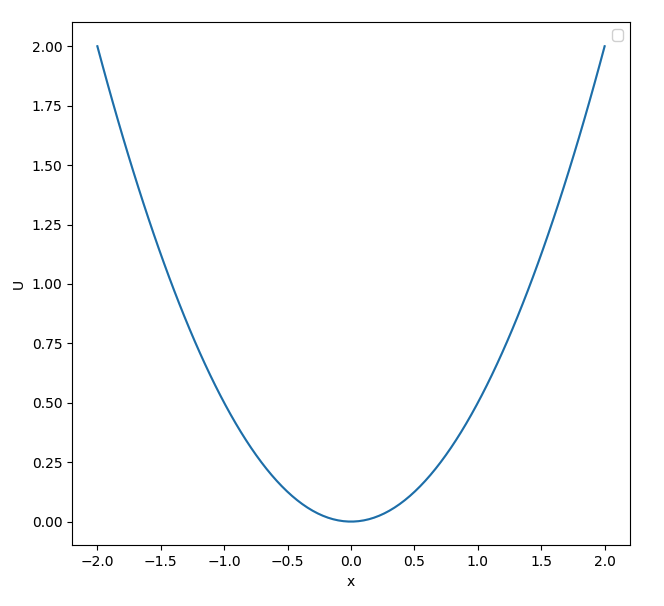
\includegraphics[scale=0.35]{ch7-7.36.png}
\end{center}
\item [\textbf{(b)}] For a classical particle the turning points happen when
$U(x) = E$ hence
\begin{align*}
    E &= \frac{1}{2}k x^2
\end{align*}
Then the turning points are 
$$x = \pm \sqrt{\frac{2E}{k}}$$
\item [\textbf{(c)}] The classically allowed region is from $-\sqrt{2E/k}$ to
$\sqrt{2E/k}$ hence the length of this region is $2\sqrt{2E/k}$.
So if we double the energy the length of the region is
$$2\sqrt{\frac{4E}{k}} = 2\sqrt{2}\sqrt{\frac{2E}{k}}$$
We see then that the length is not doubled.
\end{itemize}
\end{proof}

\cleardoublepage
\begin{proof}{\textbf{7.37}}
\begin{itemize}
\item [\textbf{(a)}] Sketch of $U$ as a function of $x$
\begin{center}
    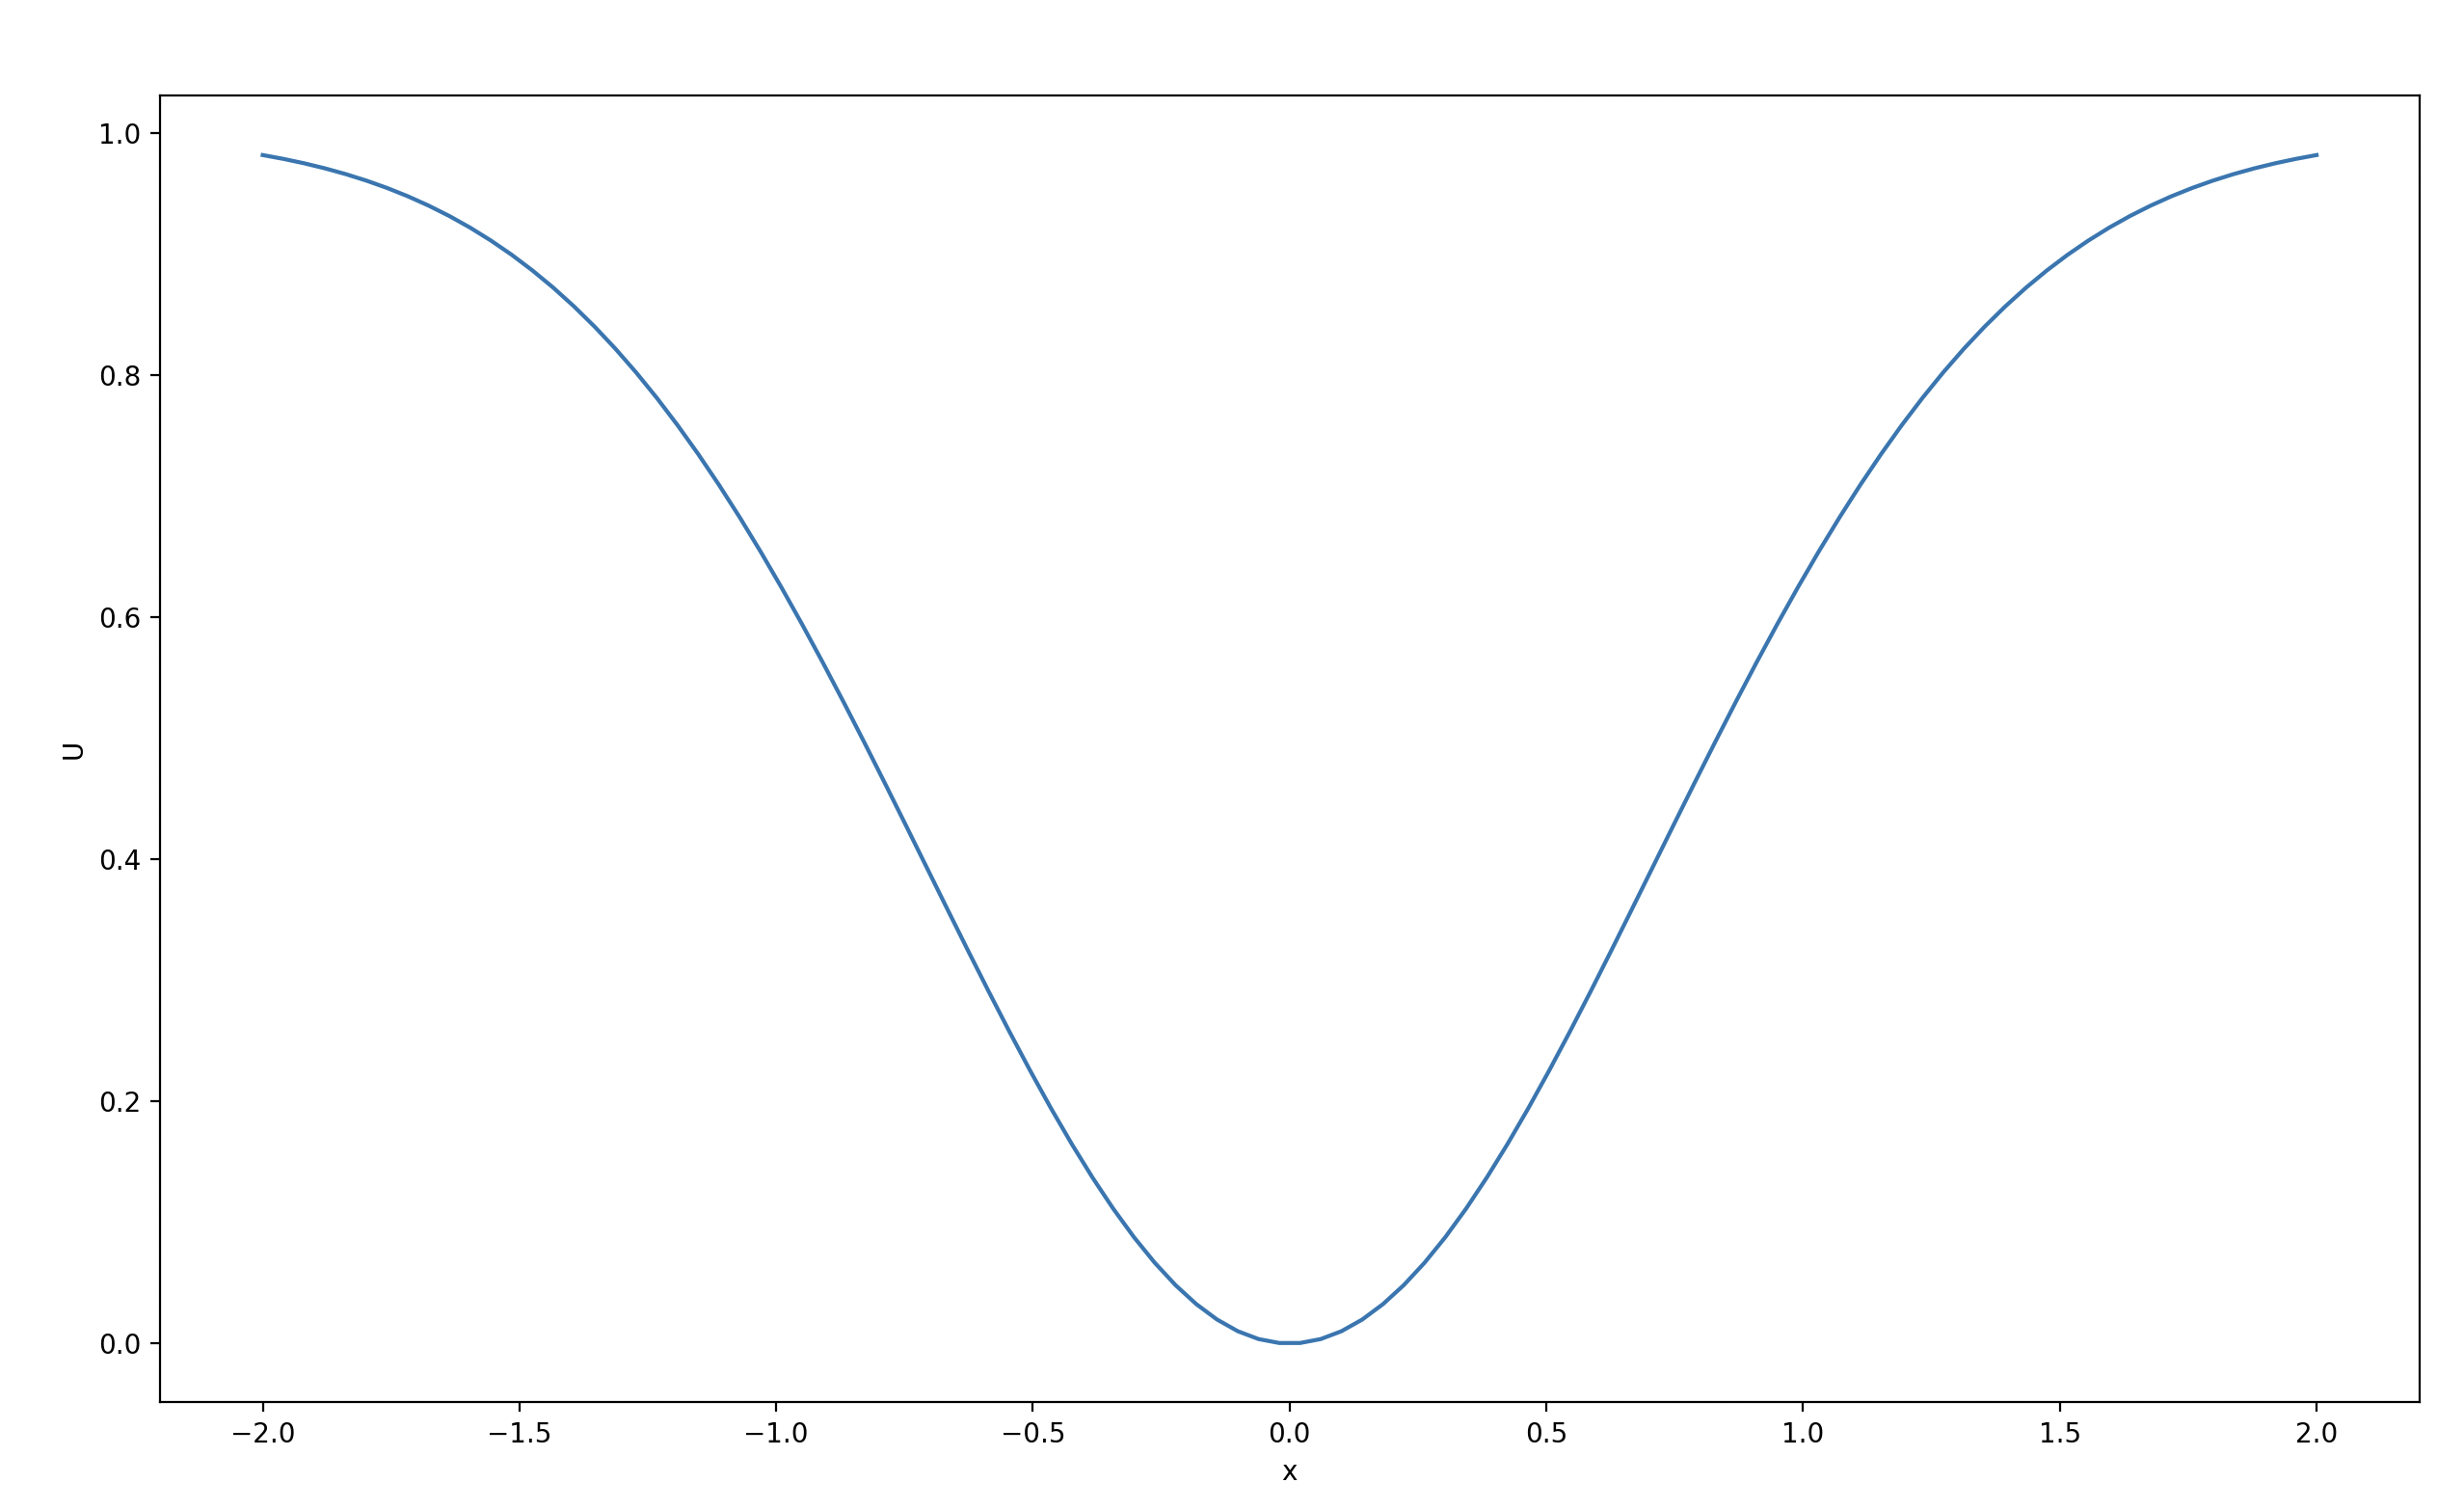
\includegraphics[scale=0.25]{ch7-7.37.png}
\end{center}

\item [\textbf{(b)}] The classical turning points happen when $U(x) = E$ hence
\begin{align*}
    E &= U_0(1 - e^{-x^2/a^2})
\end{align*}
Then the turning points are given by
\begin{align*}
    1 - e^{-x^2/a^2} &= \frac{E}{U_0}\\
    e^{-x^2/a^2} &= 1 - \frac{E}{U_0}\\
    x^2 &= -a^2\log(1 - \frac{E}{U_0})\\
    x &= \pm\sqrt{-a^2\log(1 - \frac{E}{U_0})}
\end{align*}
These tuning points are well-defined since $\log(1 - E/U_0)$ is negative for
$0 < E < U_0$ and hence the argument of the square root is positive.
\end{itemize}
\end{proof}

\cleardoublepage
\begin{proof}{\textbf{7.38}}
Let a particle moving on a finite well with an energy $E < 0$ then the
Schrödinger equation is of the form
\begin{align*}
    \psi''(x) = \text{(positive function)}\cdot \psi(x)
\end{align*}
Then $\psi(x)$ must bend away from the axis so the only physically acceptable
solution for $x > 0$ is of the form $Be^{-\alpha x}$ and for $x < 0$ should be
of the form $Ce^{\alpha x}$ where $\alpha = 2m(U_0 - E)/\hbar^2$.

Then $\psi(x)$ goes to 0 both when $x \to \infty$ and when $x \to -\infty$ then
$\psi(x)$ must have a maximum in the middle. At this maximum the function
must be concave down but this cannot happen since $\psi''(x)$ would be negative
there. Therefore there is no solution to $\psi(x)$ that is physically
acceptable.
\end{proof}

\cleardoublepage
\begin{proof}{\textbf{7.44}}
\begin{itemize}
\item [\textbf{(a)}] We know that a particle of mass $m$ in a uniform
gravitational field experiencies a force $F = -mg$ which is counteracted by the
normal force of the hard surface. Also, we know that
\begin{align*}
    F(x) = -\dv{U(x)}{x}
\end{align*}
Then by integration we have that
\begin{align*}
    U(x) = mgx
\end{align*}
Which describes the linear function of Figure 7.29.

On the other hand, if the hard surface is at the lowest potential energy, then
the potential energy must go to infinity below $0$ since the particle cannot go
below the hard surface.

\item [\textbf{(b)}] To sketch the wave functions for different states,
we analyze the Schrödinger equation, we see that for $x < 0$ the wave function
must be 0 since we have an infinitelly potential wall.

Then between $x = 0$ and $x = b$ the wave function must oscillate similar to
the case of a finite square well and when $x > b$ the wave function must decay
to 0.

Therefore the wave function for the ground state looks like
\begin{center}
    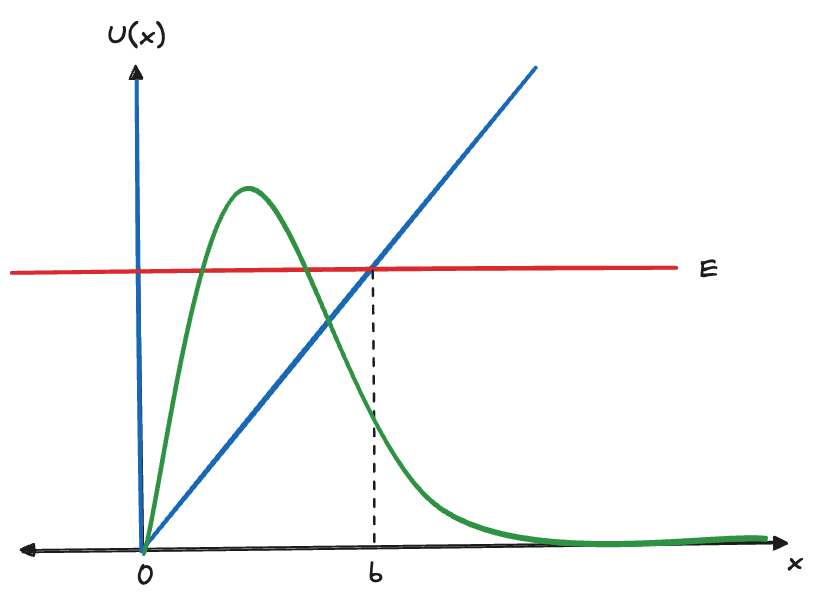
\includegraphics[scale=0.3]{ch7-7.44-i.png}
\end{center}
And for the excited states looks like
\begin{center}
    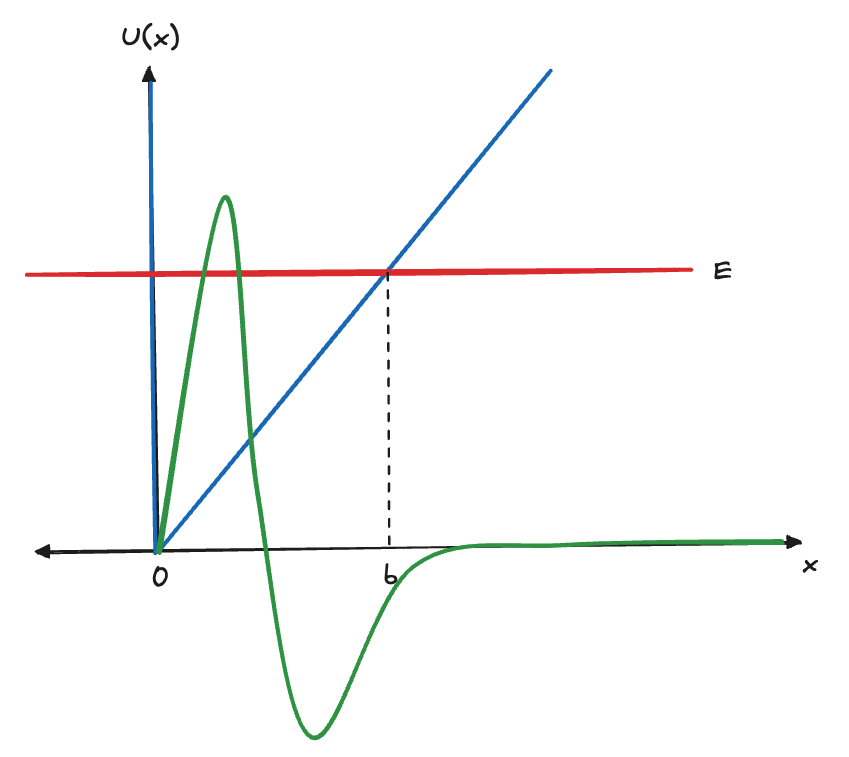
\includegraphics[scale=0.3]{ch7-7.44-ii.png}
\end{center}
\begin{center}
    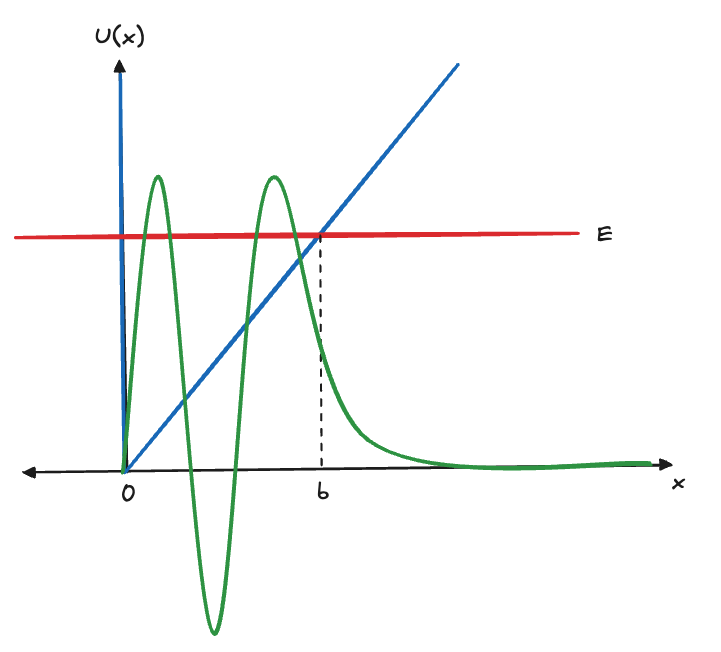
\includegraphics[scale=0.35]{ch7-7.44-iii.png}
\end{center}

\end{itemize}
\end{proof}

\cleardoublepage
\begin{proof}{\textbf{7.45}}
\begin{itemize}
\item [\textbf{(a)}] We know that the allowed energies for the infinite well
are
\begin{align*}
    E_n = n^2\frac{\pi^2\hbar^2}{2ma}
\end{align*}
If we assume that the energy of the $n$-th state of the finite well is close
to $U_0$ and that this energy is close to the $n$-th energy of the infinite
well we get that $E_n \approx U_0$ hence
\begin{align*}
    U_0 \approx n^2\frac{\pi^2\hbar^2}{2ma}
\end{align*}
Therefore
\begin{align*}
    n \approx \frac{\sqrt{2U_0ma}}{\pi\hbar}
\end{align*}

\item [\textbf{(b)}] For an electron in a well of depth $U_0 = 10~eV$ and width
$a = 0.3~nm$ the number of bound states is approximately 
\begin{align*}
    n &=
    \frac{\sqrt{2\cdot 10~eV \cdot 510998.94~eV/c^2 \cdot 0.3~nm}}
    {\pi\cdot 6.582\times 10^{-16}~eVs}\\
    &= \frac{8.4679 \times 10^{17}~nm/s}{c}\\
    &= \frac{8.4679 \times 10^{17}~nm/s}{2.998\times 10^{17}~nm/s}\\
    &= 2.82 \approx 3
\end{align*}
\end{itemize}
\end{proof}

\cleardoublepage
\begin{proof}{\textbf{7.46}}
\begin{itemize}
\item [\textbf{(a)}] The equation
$$\psi''(x) = -\psi(x)$$
Is the equation of a simple harmonic motion and we know that the solution to
this kind of equations is
$$\psi(x) = C_1\cos(x) + C_2\sin(x)$$
Then from the boundary condition $\psi(0) = 0$ must be that $C_1 = 0$.
Also, taking the derivative of $\psi(x)$ we get that 
$$\psi'(x) = C_2\cos(x)$$
So from the boundary condition $\psi'(0) = 1$ we get that $C_2 = 1$.\\
Therefore the equation for $\psi(x)$ is
$$\psi(x) = \sin(x)$$
Then the exact value of $\psi(x)$ at $x = 1$ is $\psi(1) = 0.8414$.

\item [\textbf{(b)}] Let us divide the interval from $x = 0$ to $x = 1$ into
two i.e. $\Delta x = 1/2$ then applying Euler's method we compute first
$\psi'(x_1) = \psi'(1/2)$ as follows
\begin{align*}
    \psi'(x_1) &= \psi'(x_0) + \psi''(x_0) \Delta x\\
    \psi'(1/2) &= \psi'(0) + \psi''(0) \cdot 1/2\\
    \psi'(1/2) &= 1
\end{align*}
Where we used that $\psi''(0) = -\sin(0) = 0$.\\
Now, we compute the values for $\psi(x)$ using the value we computed for
$\psi'(1/2)$ as follows
\begin{align*}
    \psi(x_1) &= \psi(x_0) + \psi'(x_0) \Delta x\\
    \psi(1/2) &= \psi(0) + \psi'(0) \cdot 1/2\\
    \psi(1/2) &= 0 + 1/2\\
    \psi(1/2) &= 1/2
\end{align*}
And
\begin{align*}
    \psi(x_2) &= \psi(x_1) + \psi'(x_1) \Delta x\\
    \psi(1) &= \psi(1/2) + \psi'(1/2) \cdot 1/2\\
    \psi(1) &= 1/2 + 1/2\\
    \psi(1) &= 1
\end{align*}
Therefore the approximation for $n = 2$ is not that close to the exact value.

\cleardoublepage
\item [\textbf{(c)}] Computing the values for $n = 3$ and $n = 4$ using a
computer we get that $\psi(1) = 0.9636$ for $n = 3$ and $\psi(1) = 0.9391$
for $n = 4$. We see that the value computed for $n = 4$ is closer to the
exact value. Using a step of $\Delta x = 0.0001$ ($n = 10000$) we can agree
with the exact value to four digits.

Finally, below we compare the approximated values of $\psi(x)$ for $n = 4$
to the exact value.
\begin{center}
    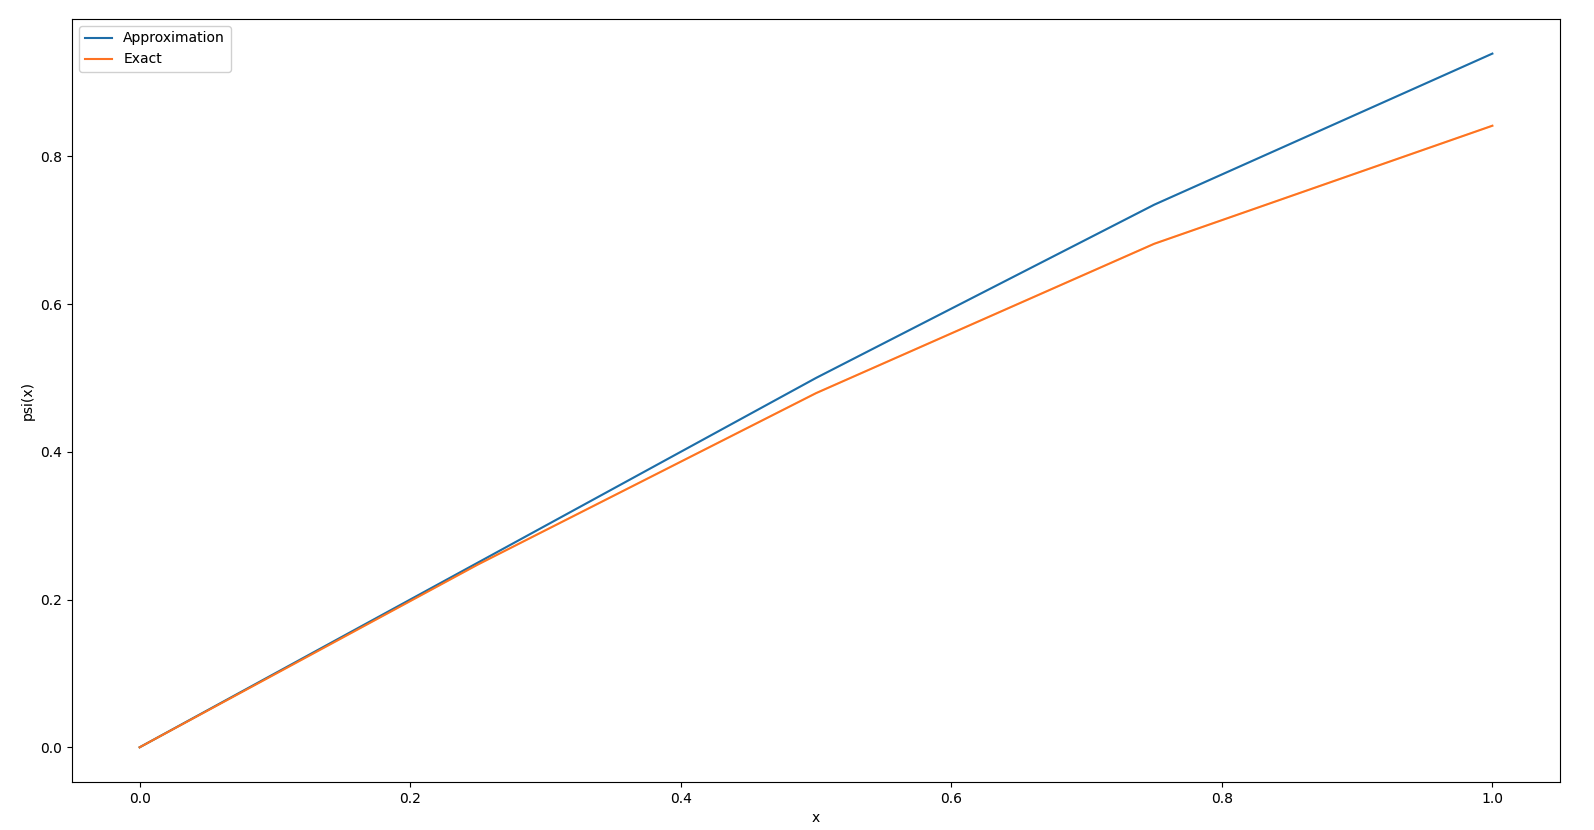
\includegraphics[scale=0.215]{ch7-7.46.png}
\end{center} 
\end{itemize}
\end{proof}


\cleardoublepage
\begin{proof}{\textbf{7.47}}
\begin{itemize}
\item [\textbf{(a)}] The equation
$$\psi''(x) = \psi(x)$$
Has the following general solution
$$\psi(x) = C_1e^x + C_2e^{-x}$$
Then from the boundary condition $\psi(0) = 0$ must be that $C_1 = -C_2$.
Also, taking the derivative of $\psi(x)$ we get that 
$$\psi'(x) = C_1e^x - C_2e^{-x}$$
So from the boundary condition $\psi'(0) = 1$ we get that $C_1 = 1/2$
and hence $C_2 = -1/2$.\\
Therefore the equation for $\psi(x)$ is
$$\psi(x) = \frac{e^x}{2} - \frac{e^{-x}}{2}$$
Then the exact value of $\psi(x)$ at $x = 1$ is $\psi(1) = 1.1752$.

\item [\textbf{(b)}] Let us divide the interval from $x = 0$ to $x = 1$ into
two i.e. $\Delta x = 1/2$ then applying Euler's method we compute first
$\psi'(x_1) = \psi'(1/2)$ as follows
\begin{align*}
    \psi'(x_1) &= \psi'(x_0) + \psi''(x_0) \Delta x\\
    \psi'(1/2) &= \psi'(0) + \psi''(0) \cdot 1/2\\
    \psi'(1/2) &= 1
\end{align*}
Where we used that $\psi''(0) = 0$.\\
Now, we compute the values for $\psi(x)$ using the value we computed for
$\psi'(1/2)$ as follows
\begin{align*}
    \psi(x_1) &= \psi(x_0) + \psi'(x_0) \Delta x\\
    \psi(1/2) &= \psi(0) + \psi'(0) \cdot 1/2\\
    \psi(1/2) &= 0 + 1/2\\
    \psi(1/2) &= 1/2
\end{align*}
And
\begin{align*}
    \psi(x_2) &= \psi(x_1) + \psi'(x_1) \Delta x\\
    \psi(1) &= \psi(1/2) + \psi'(1/2) \cdot 1/2\\
    \psi(1) &= 1/2 + 1/2\\
    \psi(1) &= 1
\end{align*}
Therefore the approximation for $n = 2$ is not that close to the exact value.

\cleardoublepage
\item [\textbf{(c)}] Computing the values for $n = 3$ and $n = 4$ using a
computer we get that $\psi(1) = 1.0641$ for $n = 3$ and $\psi(1) = 1.0377$
for $n = 4$. We see that the value computed for $n = 3$ is closer to the
exact value compared to the value computed for $n = 4$.

Finally, below we compare the approximated values of $\psi(x)$ for
$n = 3$, $n = 4$ and $n = 100$ to the exact value.
\begin{center}
    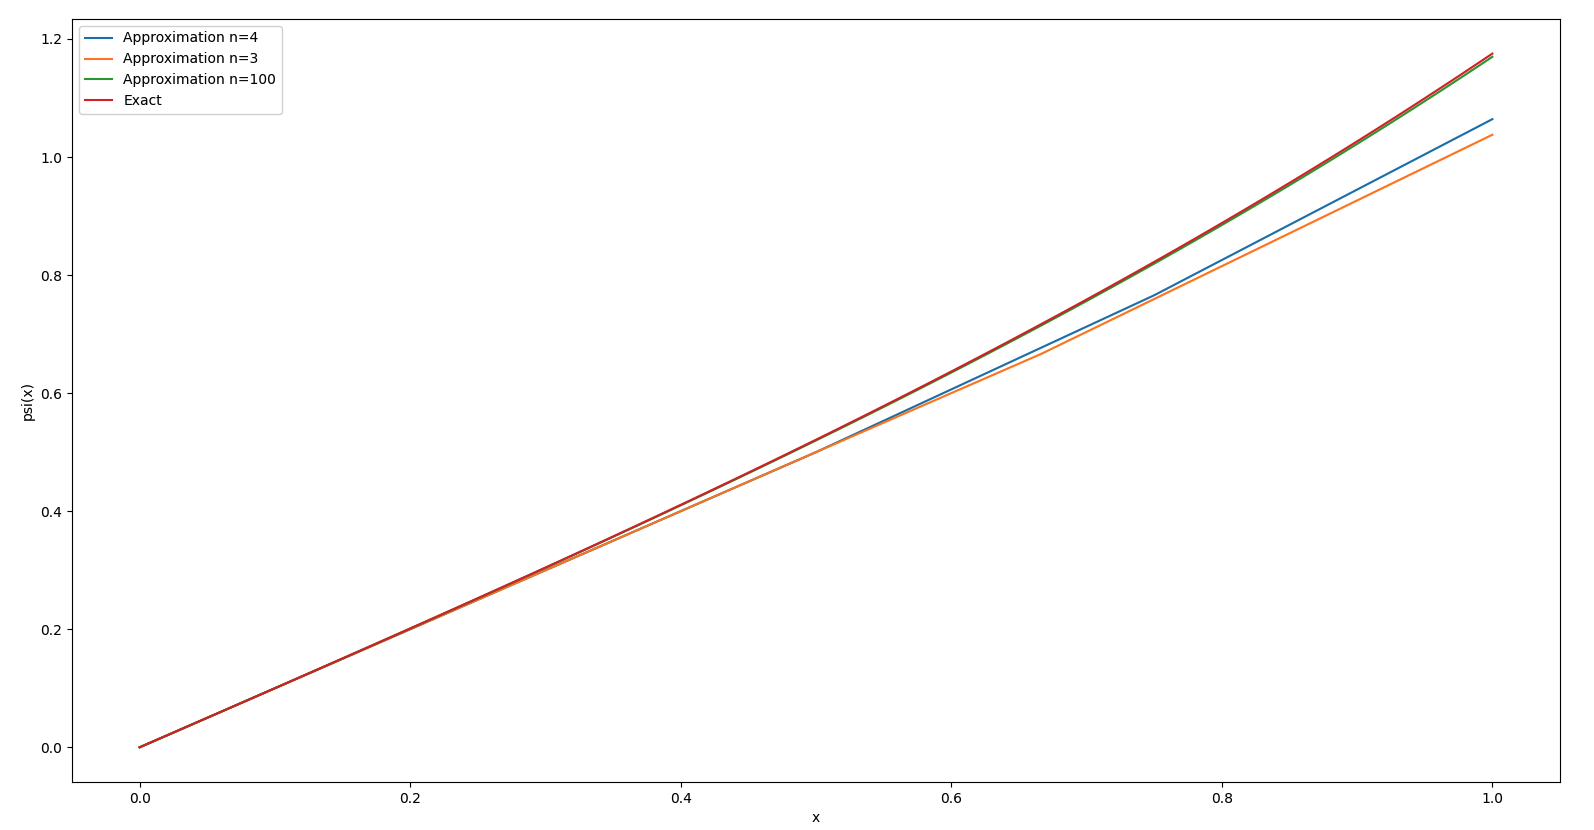
\includegraphics[scale=0.215]{ch7-7.47.png}
\end{center} 
\end{itemize}
\end{proof}

\cleardoublepage
\begin{proof}{\textbf{7.48}}
Let a particle with the energy of the quantum ground state
$E = \hbar \omega_c / 2$. We know that at the classical turning point
$x = \pm a$ and we determined that $a = \sqrt{2E/k}$ hence we have that
\begin{align*}
    x = a  = \sqrt{\frac{2E}{k}} = \sqrt{\frac{\hbar\omega_c}{m \omega_c^2}}
    = \sqrt{\frac{\hbar}{m \omega_c}}
\end{align*}
Where we used that $k = m \omega_c^2$.
\end{proof}

\cleardoublepage
\begin{proof}{\textbf{7.53}}
\begin{itemize}
\item [\textbf{(a)}]
We know that the position of a classical particle is given by
\begin{align*}
    x = a\sin\omega_c t
\end{align*}
So the turning points happen at $x = \pm a$ but since at $x = a$ all its energy
is potential energy then $E = \frac{1}{2}ka^2$ and hence
\begin{align*}
    a = \pm \sqrt{\frac{2E}{k}}
\end{align*}
But we are considering a particle in the ground state
$E = \frac{1}{2}\hbar \omega_c$ so the turning points happen at
\begin{align*}
    a = \pm \sqrt{\frac{\hbar \omega_c}{k}}
\end{align*}
Or in terms of $b$ using that $k = m\omega_c^2$ we get that
\begin{align*}
    a = \pm \sqrt{\frac{\hbar \omega_c}{m \omega_c^2}}
    = \pm \sqrt{\frac{\hbar}{m \omega_c}}
    = \pm b
\end{align*}
\item [\textbf{(b)}] The probability of finding the particle between
the two classical turning points is given by
\begin{align*}
    \int_{-a}^a |\psi(x)|^2~dx 
    &= \int_{-b}^{b} |(\pi b^2)^{-1/4} e^{-x^2/2b^2}|^2~dx\\
    &= \frac{1}{b\sqrt{\pi}} \int_{-b}^{b} |e^{-x^2/2b^2}|^2~dx\\
    &= \frac{1}{b\sqrt{\pi}} \int_{-1}^{1} |e^{-y^2/2}|^2b~dy\\
    &= \frac{1}{\sqrt{\pi}} \int_{-1}^{1} e^{-y^2}~dy\\
    &= \frac{1.49}{\sqrt{\pi}} = 0.84
\end{align*}
Where we changed variables defining $y = x/b$ so $dx = b~dy$. 
\item [\textbf{(c)}] Since the probability of finding the particle anywhere
must be $1$ and we know that the probability of finding the particle between
the classical turning points is $0.84$ then the probability of finding the
particle outside the classical turning points must be $1 - 0.84 = 0.16$.
\end{itemize}
\end{proof}

\cleardoublepage
\begin{proof}{\textbf{7.54}}
Let two straight wires lying on the $x$ axis separated by a gap of $L = 4~nm$
such that $U_0 - E = 3~eV$ then $\alpha$ in this case is 
\begin{align*}
    \alpha &= \frac{\sqrt{2mc^2(U_0 - E)}}{\hbar c}\\
    &= \frac{\sqrt{2 \cdot 5\sci{5}~eV\cdot 3~eV}}{197~eV~nm}\\
    &= 8.79~nm^{-1}
\end{align*}
Then $\alpha L = 8.79~nm^{-1} \cdot 4~nm = 35.16$ hence the probability that a
conduction electron in one wire arriving at the gap will pass through the gap is
\begin{align*}
    P = e^{-2\alpha L} = e^{-70.32} = 2.88 \sci{-31}
\end{align*}
\end{proof}
\begin{proof}{\textbf{7.55}}
Let a barrier width of $L = 35~fm = 35 \sci{-5}~nm$ and $U_0 - E = 5~MeV$ then
$\alpha$ in this case is
\begin{align*}
    \alpha &= \frac{\sqrt{2mc^2(U_0 - E)}}{\hbar c}\\
    &= \frac{\sqrt{2 \cdot 3.73\sci{9}~eV\cdot 5\sci{6}~eV}}{197~eV~nm}\\
    &= 980365.88~nm^{-1}
\end{align*}
Where we used that $mc^2 = 3.73\sci{9}~eV$ for an alpha particle.
\\
Then $\alpha L = 980365.88~nm^{-1} \cdot 3.5\sci{-5}~nm = 34.31$ hence
the probability of an alpha particle hitting the nuclear surface and escaping
is
\begin{align*}
    P = e^{-2\alpha L} = e^{-68.62} = 1.58 \sci{-30}
\end{align*}
Given that the alpha particle hits the nuclear surface about $5\sci{21}$ times
per second, the probability that it will escape in a day is
\begin{align*}
    1.58 \sci{-30} \cdot 86400 \cdot 5\sci{21} = 0.0007 = 0.07 \%
\end{align*}
Where we used that the particle hits the nucleus $86400 \cdot 5\sci{21}$ a day.
\end{proof}

\cleardoublepage
\begin{proof}{\textbf{7.57}}
Let $\psi(x)$ be a wave function that satisfies the time-independent
Schrödinger equation. We want to prove that $\Psi(x,t) = \psi(x)e^{-iEt/\hbar}$
satisfies the time-dependent Schrödinger equation then replacing, we see that
\begin{align*}
    i\hbar \pdv{t}\psi(x)e^{-iEt/\hbar}
    &= -\frac{\hbar^2}{2m}\pdv[2]{x}\psi(x) e^{-iEt/\hbar}
    + U(x)\psi(x)e^{-iEt/\hbar}\\
    E\psi(x) e^{-iEt/\hbar}
    &= -\frac{\hbar^2}{2m}e^{-iEt/\hbar}\pdv[2]{x}\psi(x)
    + U(x)\psi(x)e^{-iEt/\hbar}\\
    E\psi(x) &= - \frac{\hbar^2}{2m}\pdv[2]{x}\psi(x) + U(x)\psi(x)\\
    \pdv[2]{x}\psi(x) &= \frac{2m}{\hbar^2}[U(x) - E]\psi(x)
\end{align*}
So the time-dependent Schrödinger equation becomes the time-independent
Schrödinger equation and we know that $\psi(x)$ satisfies it, therefore
$\Psi(x,t) = \psi(x)e^{-iEt/\hbar}$ satisfies the time-dependent Schrödinger
equation.
\end{proof}

\cleardoublepage
\begin{proof}{\textbf{7.58}}
Let $\psi_1(x)$ and $\psi_2(x)$ be the lowest two wave functions of the rigid
box. We know that
\begin{align*}
    \int_0^a |\psi_1(x)|^2~dx = 1 \qquad \int_0^a |\psi_2(x)|^2~dx = 1
\end{align*}
We want to prove first that $\int_0^a \psi_1(x)\psi_2(x)~dx = 0$ so we do as
follows
\begin{align*}
    \int_0^a \psi_1(x)\psi_2(x)~dx
    &= \int_0^a \sqrt{\frac{2}{a}}\sin(\frac{\pi x}{a})
    \sqrt{\frac{2}{a}}\sin(\frac{2\pi x}{a})~dx\\
    &= \frac{2}{a} \int_0^a \sin(\frac{\pi x}{a})\sin(\frac{2\pi x}{a})~dx\\
    &= \frac{4}{3\pi } \bigg[\sin^3\bigg(\frac{\pi x}{a}\bigg)\bigg]_0^a\\
    &= \frac{4}{3\pi } \bigg[\sin^3(\pi) - \sin^3(0)\bigg]\\
    &= 0
\end{align*}
Now, we can check that the superposition (7.114) is normalized
\begin{align*}
\int_0^a |\Psi(x)|^2~dx
&= \int_0^a \frac{1}{2}|\psi_1(x) + \psi_2(x)e^{-i\omega_{21}t}|^2~dx\\
&= \int_0^a \frac{1}{2}[\psi_1(x)^2 + \psi_2(x)^2 + 2\psi_1(x)\psi(x)\cos(\omega_{21}t)]~dx\\
&= \frac{1}{2}\bigg[
    \int_0^a \psi_1(x)^2~dx
    + \int_0^a \psi_2(x)^2~dx
    + 2\cos(\omega_{21}t)\int_{0}^a \psi_1(x)\psi(x)~dx
\bigg]\\
&= \frac{1}{2}[1 + 1 + 0]\\
&= 1 
\end{align*}
Therefore $\Psi(x)$ is normalized as we wanted.
\end{proof}

\cleardoublepage
\begin{proof}{\textbf{7.59}}
Let us compute $|\Psi(x,t)|^2$ for the wave function (7.111), then
\begin{align*}
    |\Psi(x,t)|^2
    &= |\alpha\psi_1(x)e^{-i\omega_1t} + \beta\psi_2(x)e^{-i\omega_2t}|^2\\
    &= (\alpha\psi_1(x)e^{-i\omega_1t} + \beta\psi_2(x)e^{-i\omega_2t})
    \overline{(\alpha\psi_1(x)e^{-i\omega_1t} + \beta\psi_2(x)e^{-i\omega_2t})}\\
    %
    &= \alpha\psi_1(x)e^{-i\omega_1t}\overline{\alpha\psi_1(x)e^{-i\omega_1t}}
    + \beta\psi_2(x)e^{-i\omega_2t}\overline{\beta\psi_2(x)e^{-i\omega_2t}}\\
    &\quad+ \alpha\psi_1(x)e^{-i\omega_1t}\overline{\beta\psi_2(x)e^{-i\omega_2t}}
    + \beta\psi_2(x)e^{-i\omega_2t}\overline{\alpha\psi_1(x)e^{-i\omega_1t}}\\
    %
    &= |\alpha|^2\psi_1^2(x) + |\beta|^2\psi_2^2(x)
    + \alpha\overline{\beta}\psi_1(x)\psi_2(x)e^{i(\omega_2-\omega_1)t}
   + \beta\overline{\alpha}\psi_1(x)\psi_2(x)e^{i(\omega_1-\omega_2)t}\\
    %
    &= |\alpha|^2\psi_1^2(x) + |\beta|^2\psi_2^2(x)
    + 2\Re(\alpha\overline{\beta}e^{i(\omega_2-\omega_1)t})\psi_1(x)\psi_2(x)
\end{align*}
\end{proof}

\cleardoublepage
\begin{proof}{\textbf{7.60}}\\
    The standing wave is at full amplitude $(A = 1)$ at $t = 0$ and then
    decreases as times passes.
    \begin{center}
        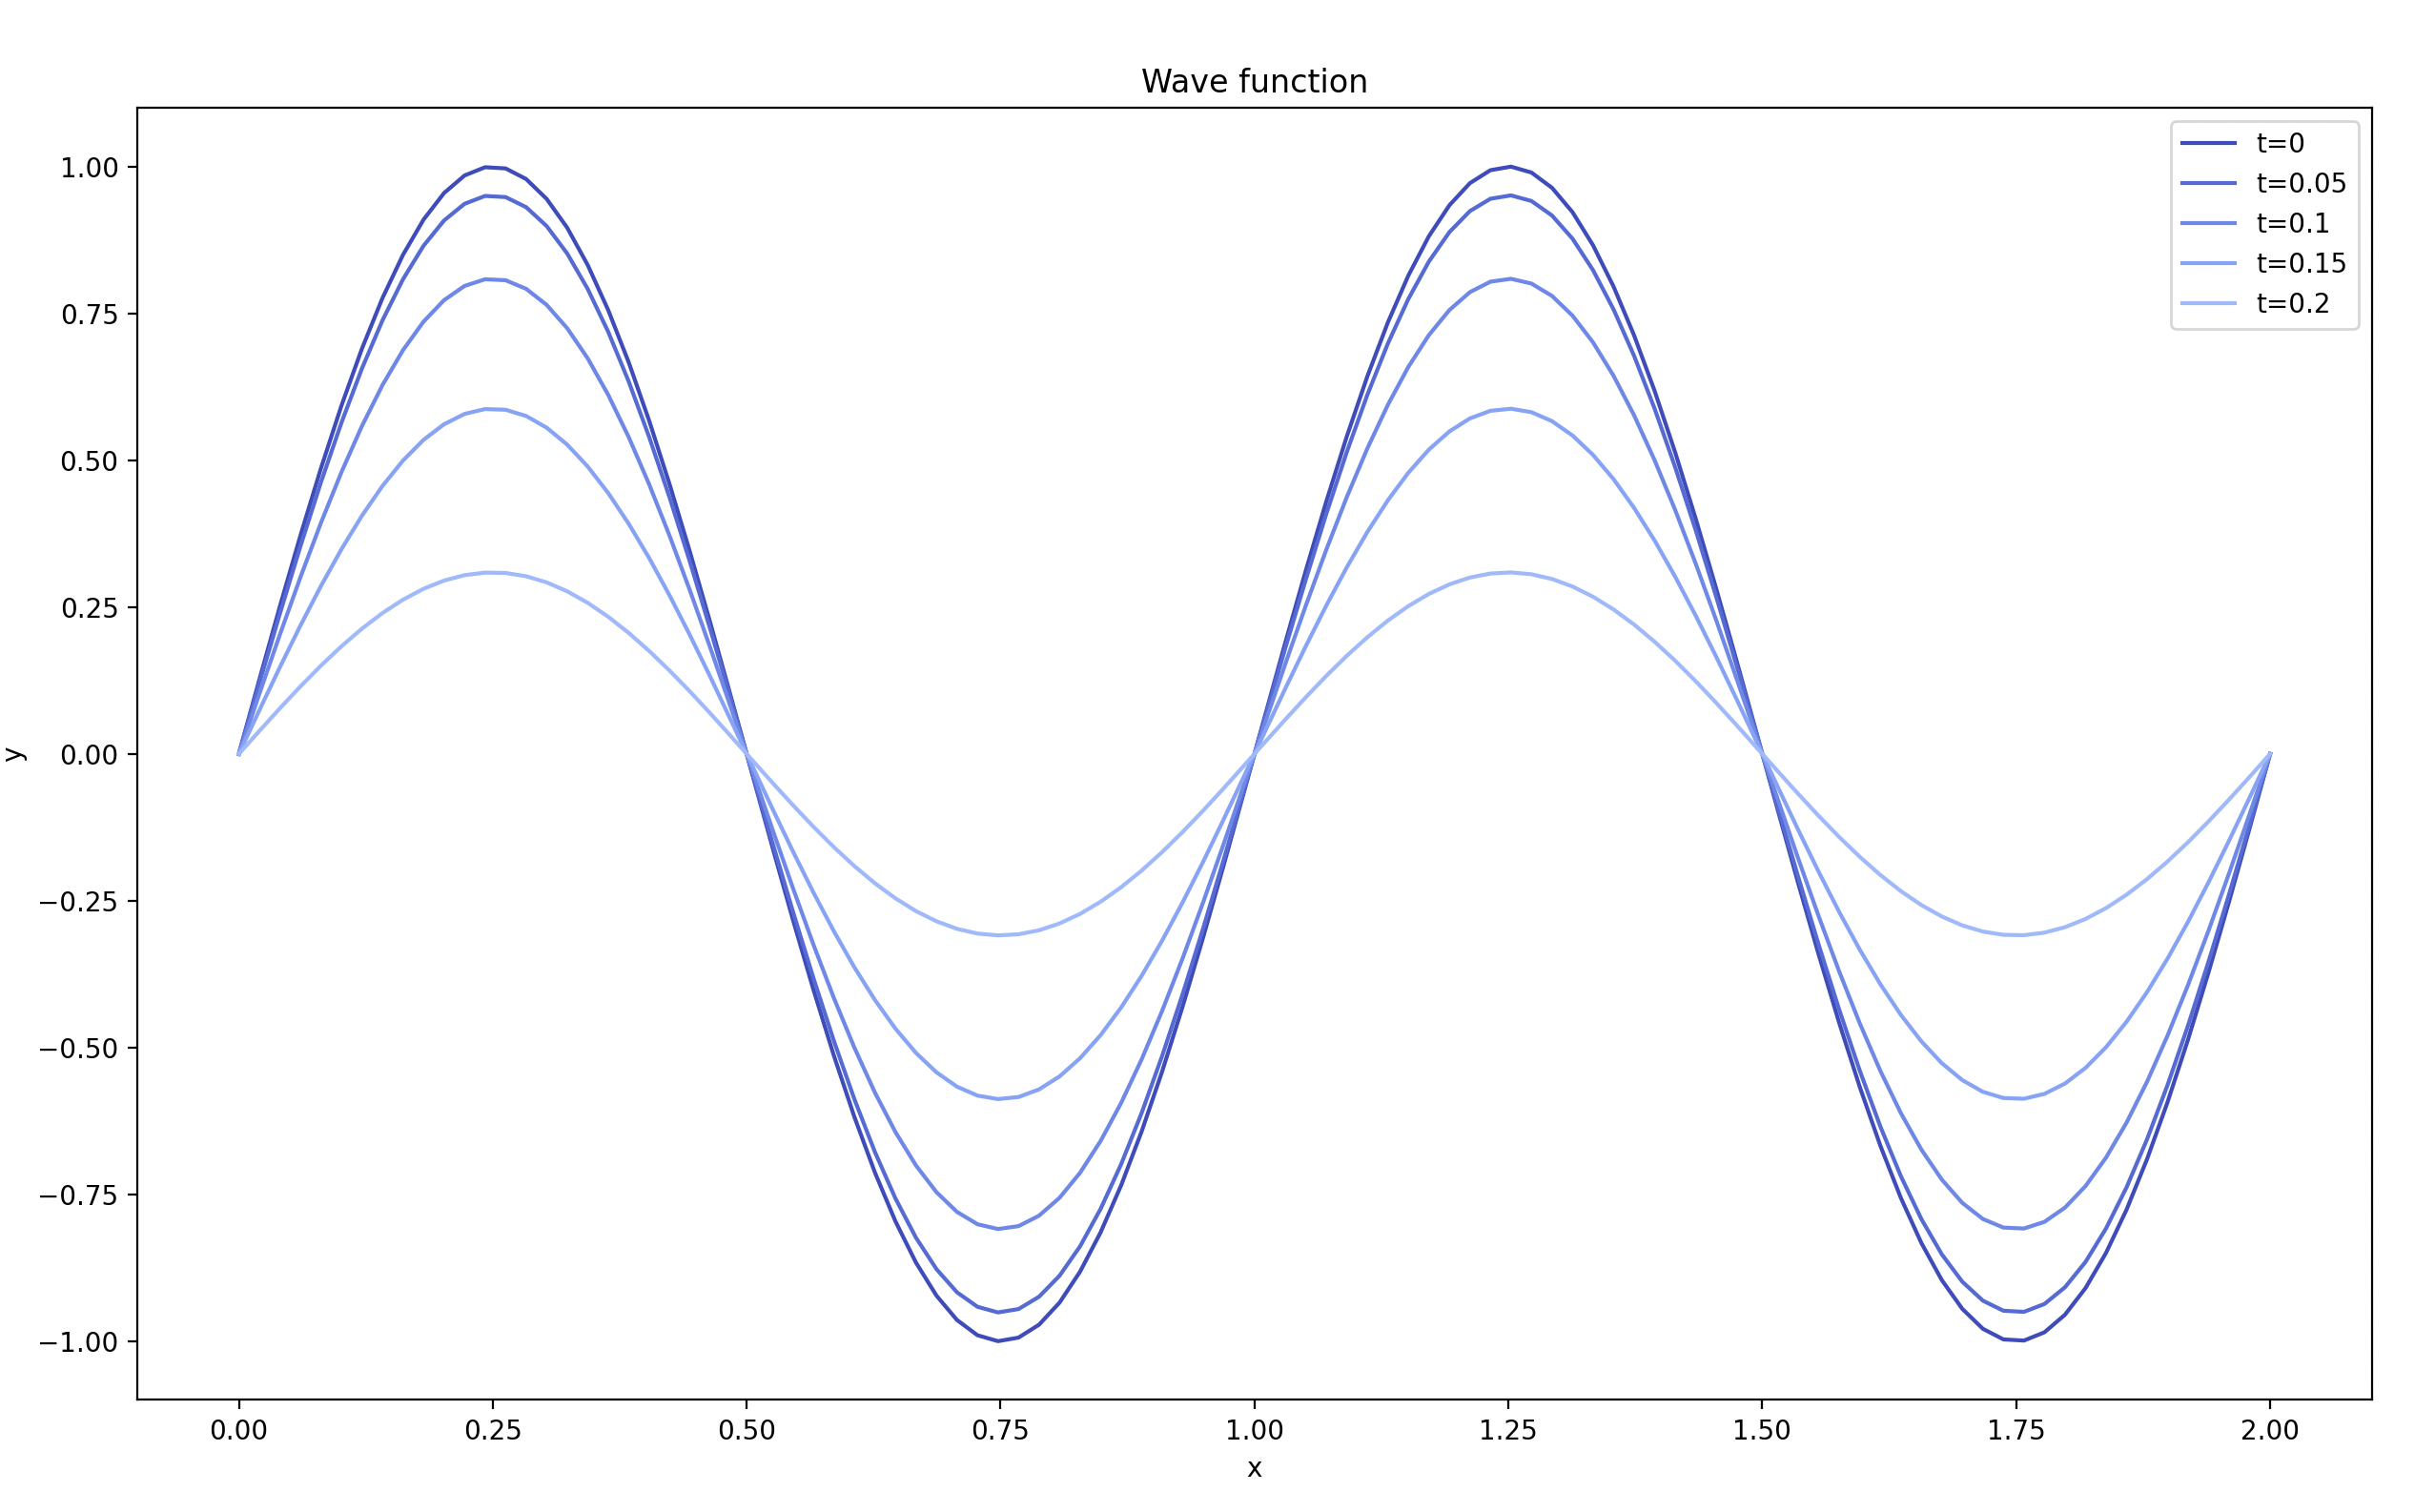
\includegraphics[scale=0.25]{ch7-7.60.png}
    \end{center}
\end{proof}
\begin{proof}{\textbf{7.61}}\\
Below we show a plot of the lowest two wave functions of the simple harmonic
oscillator
\begin{center}
    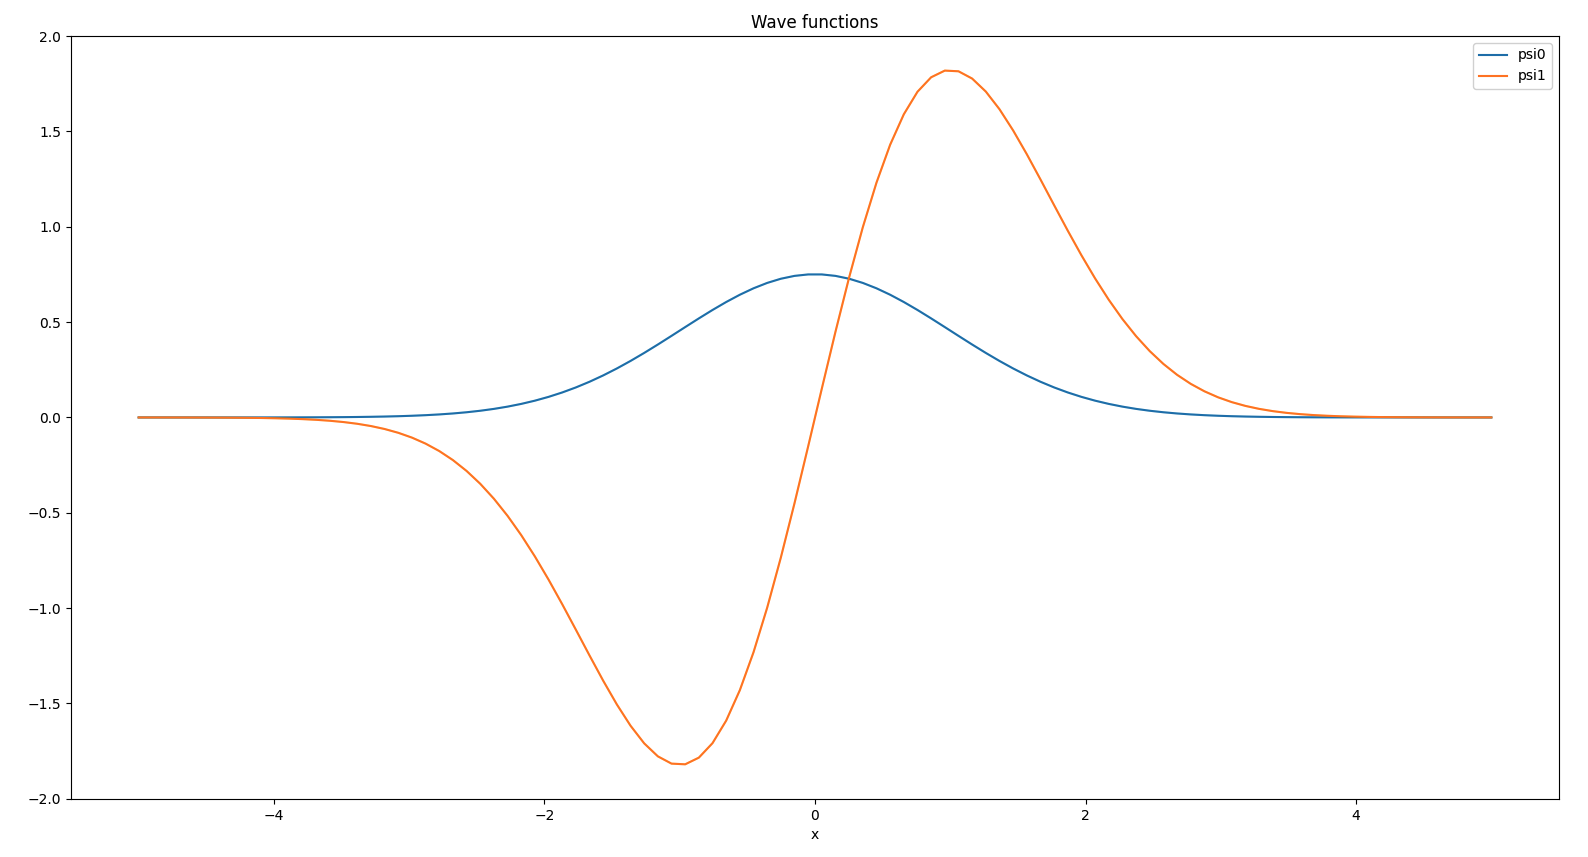
\includegraphics[scale=0.24]{ch7-7.61.png}
\end{center}
\end{proof}
\begin{proof}{\textbf{7.62}}
    Executing \verb|ch7-7.62.py| file the required animation can be generated.
\end{proof}
\begin{proof}{\textbf{7.63}}
    Executing \verb|ch7-7.63.py| file the required animation can be generated.
\end{proof}


\cleardoublepage
\begin{proof}{\textbf{7.64}}
The plot was generated using the file \verb|ch7-7.64-65.py|.
\begin{center}
    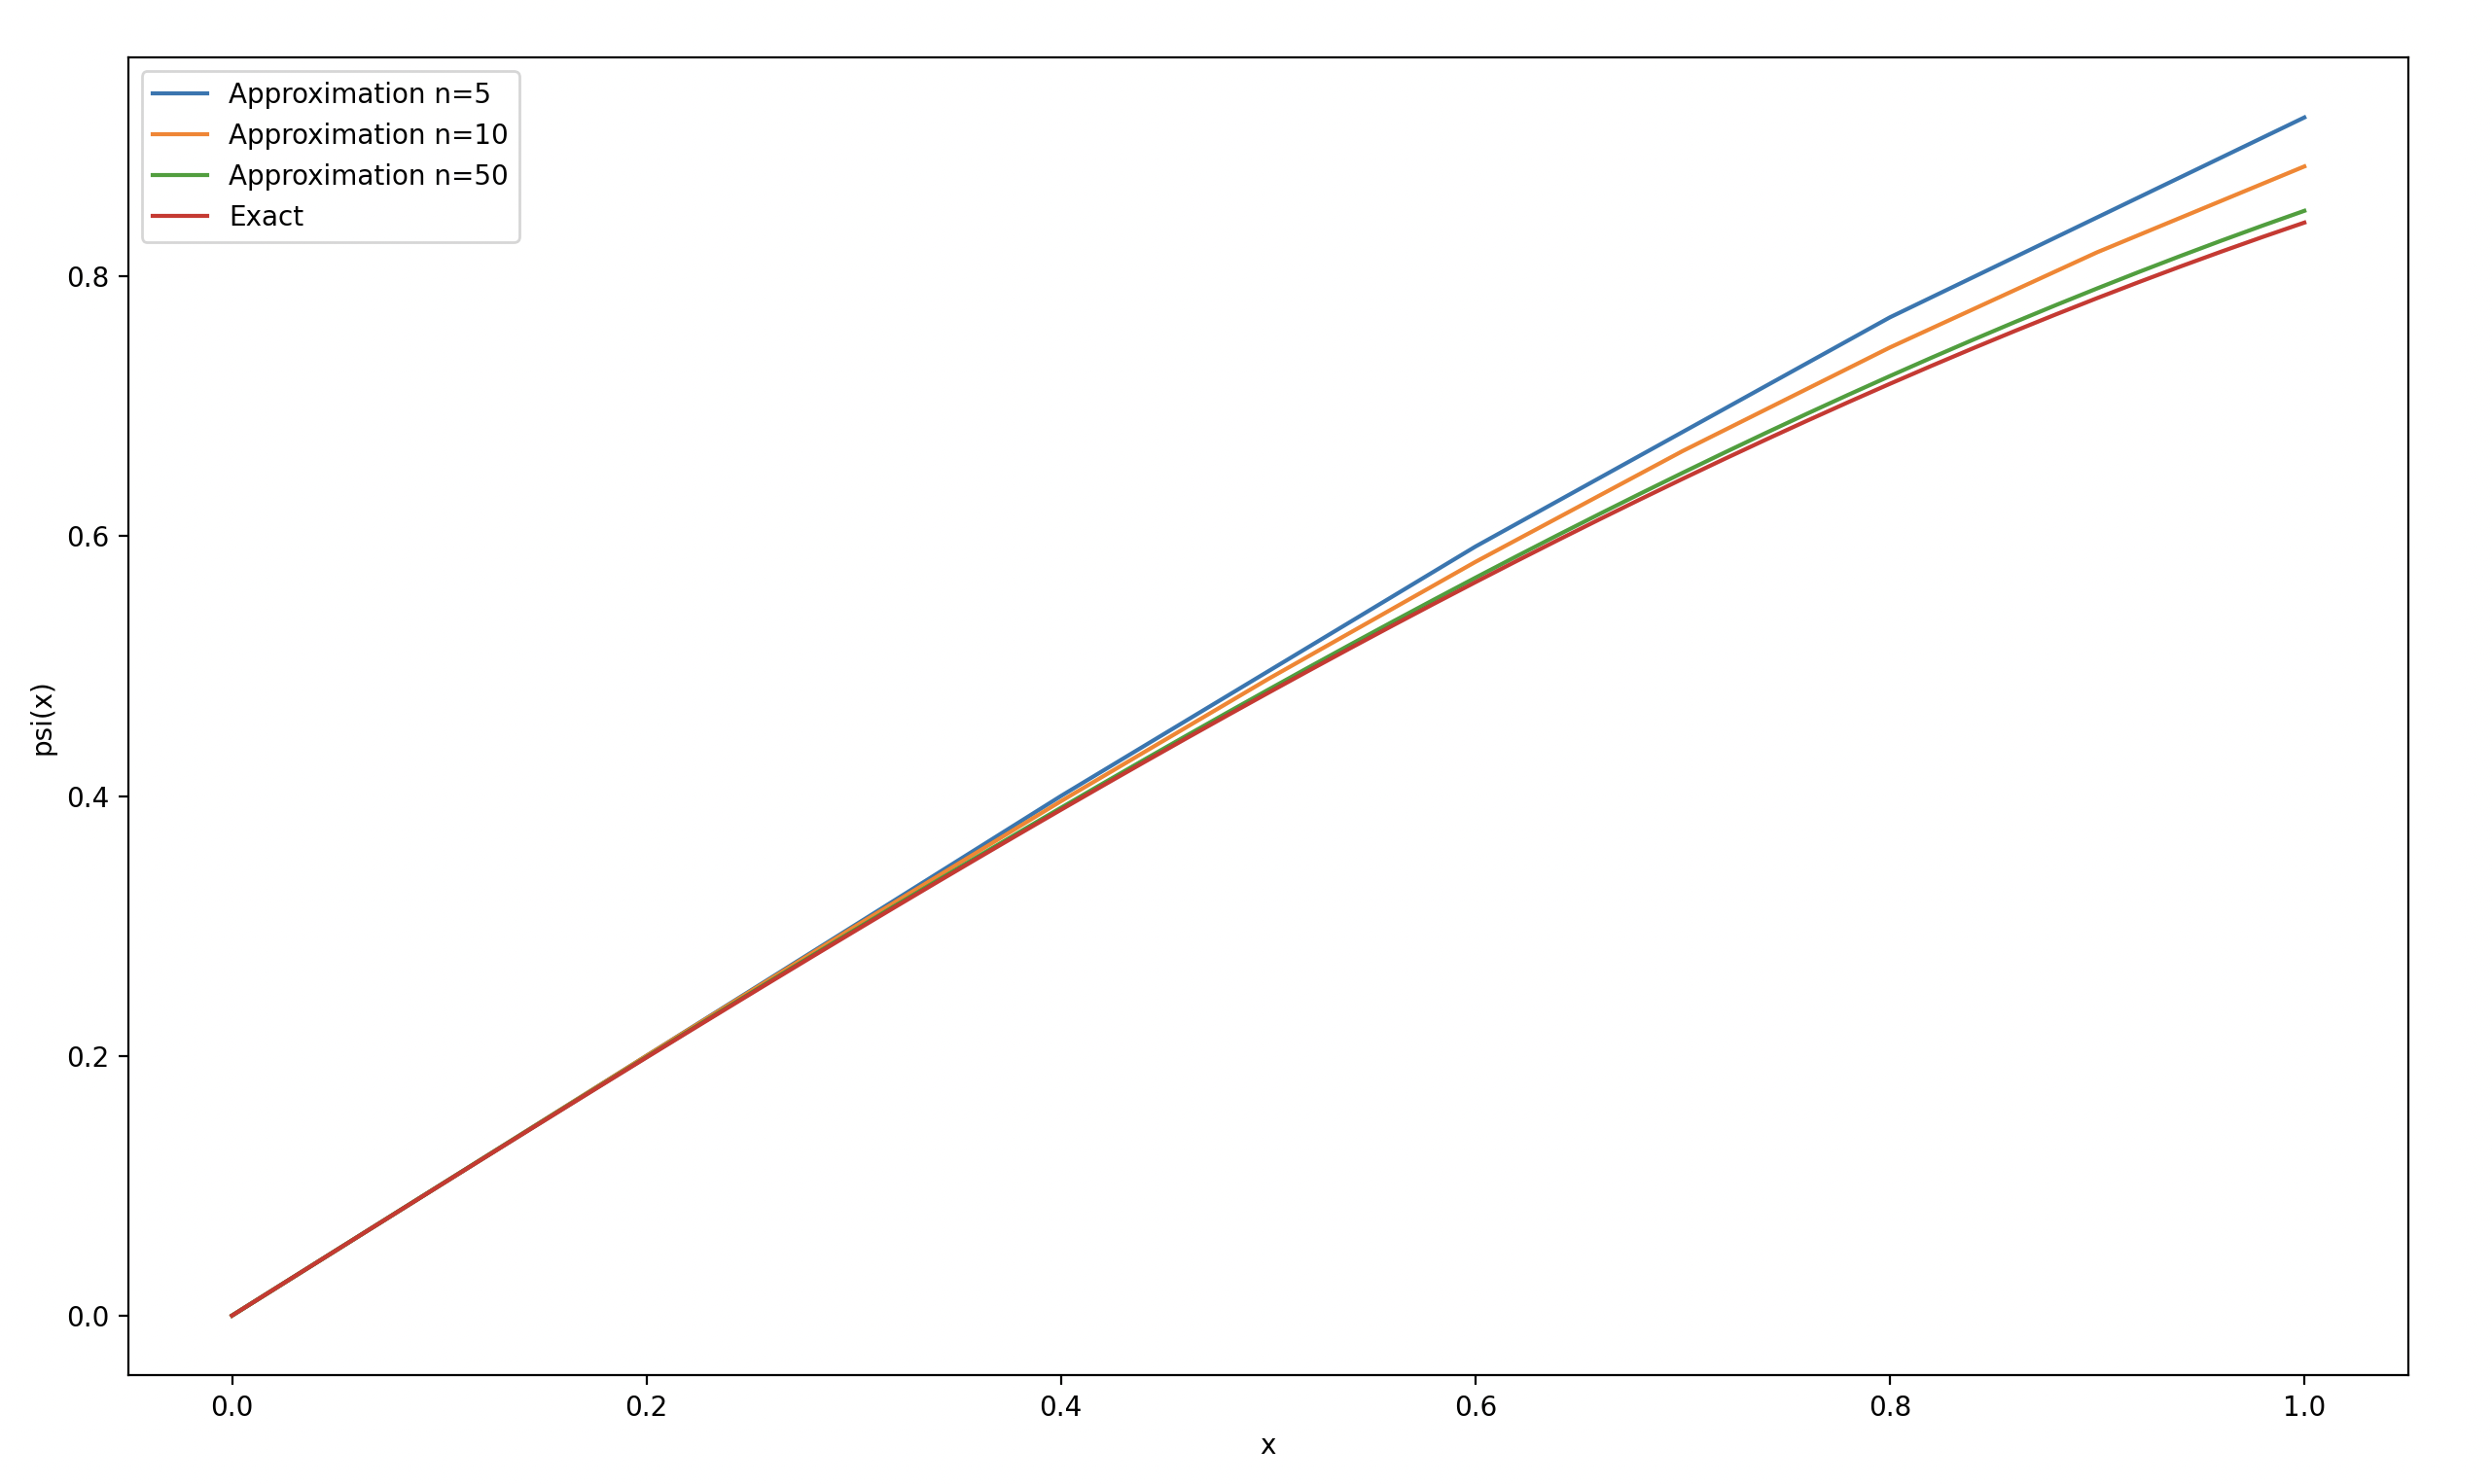
\includegraphics[scale=0.215]{ch7-7.64.png}
\end{center} 
\end{proof}
\begin{proof}{\textbf{7.65}}
The plot was generated using the file \verb|ch7-7.64-65.py|.
\begin{center}
    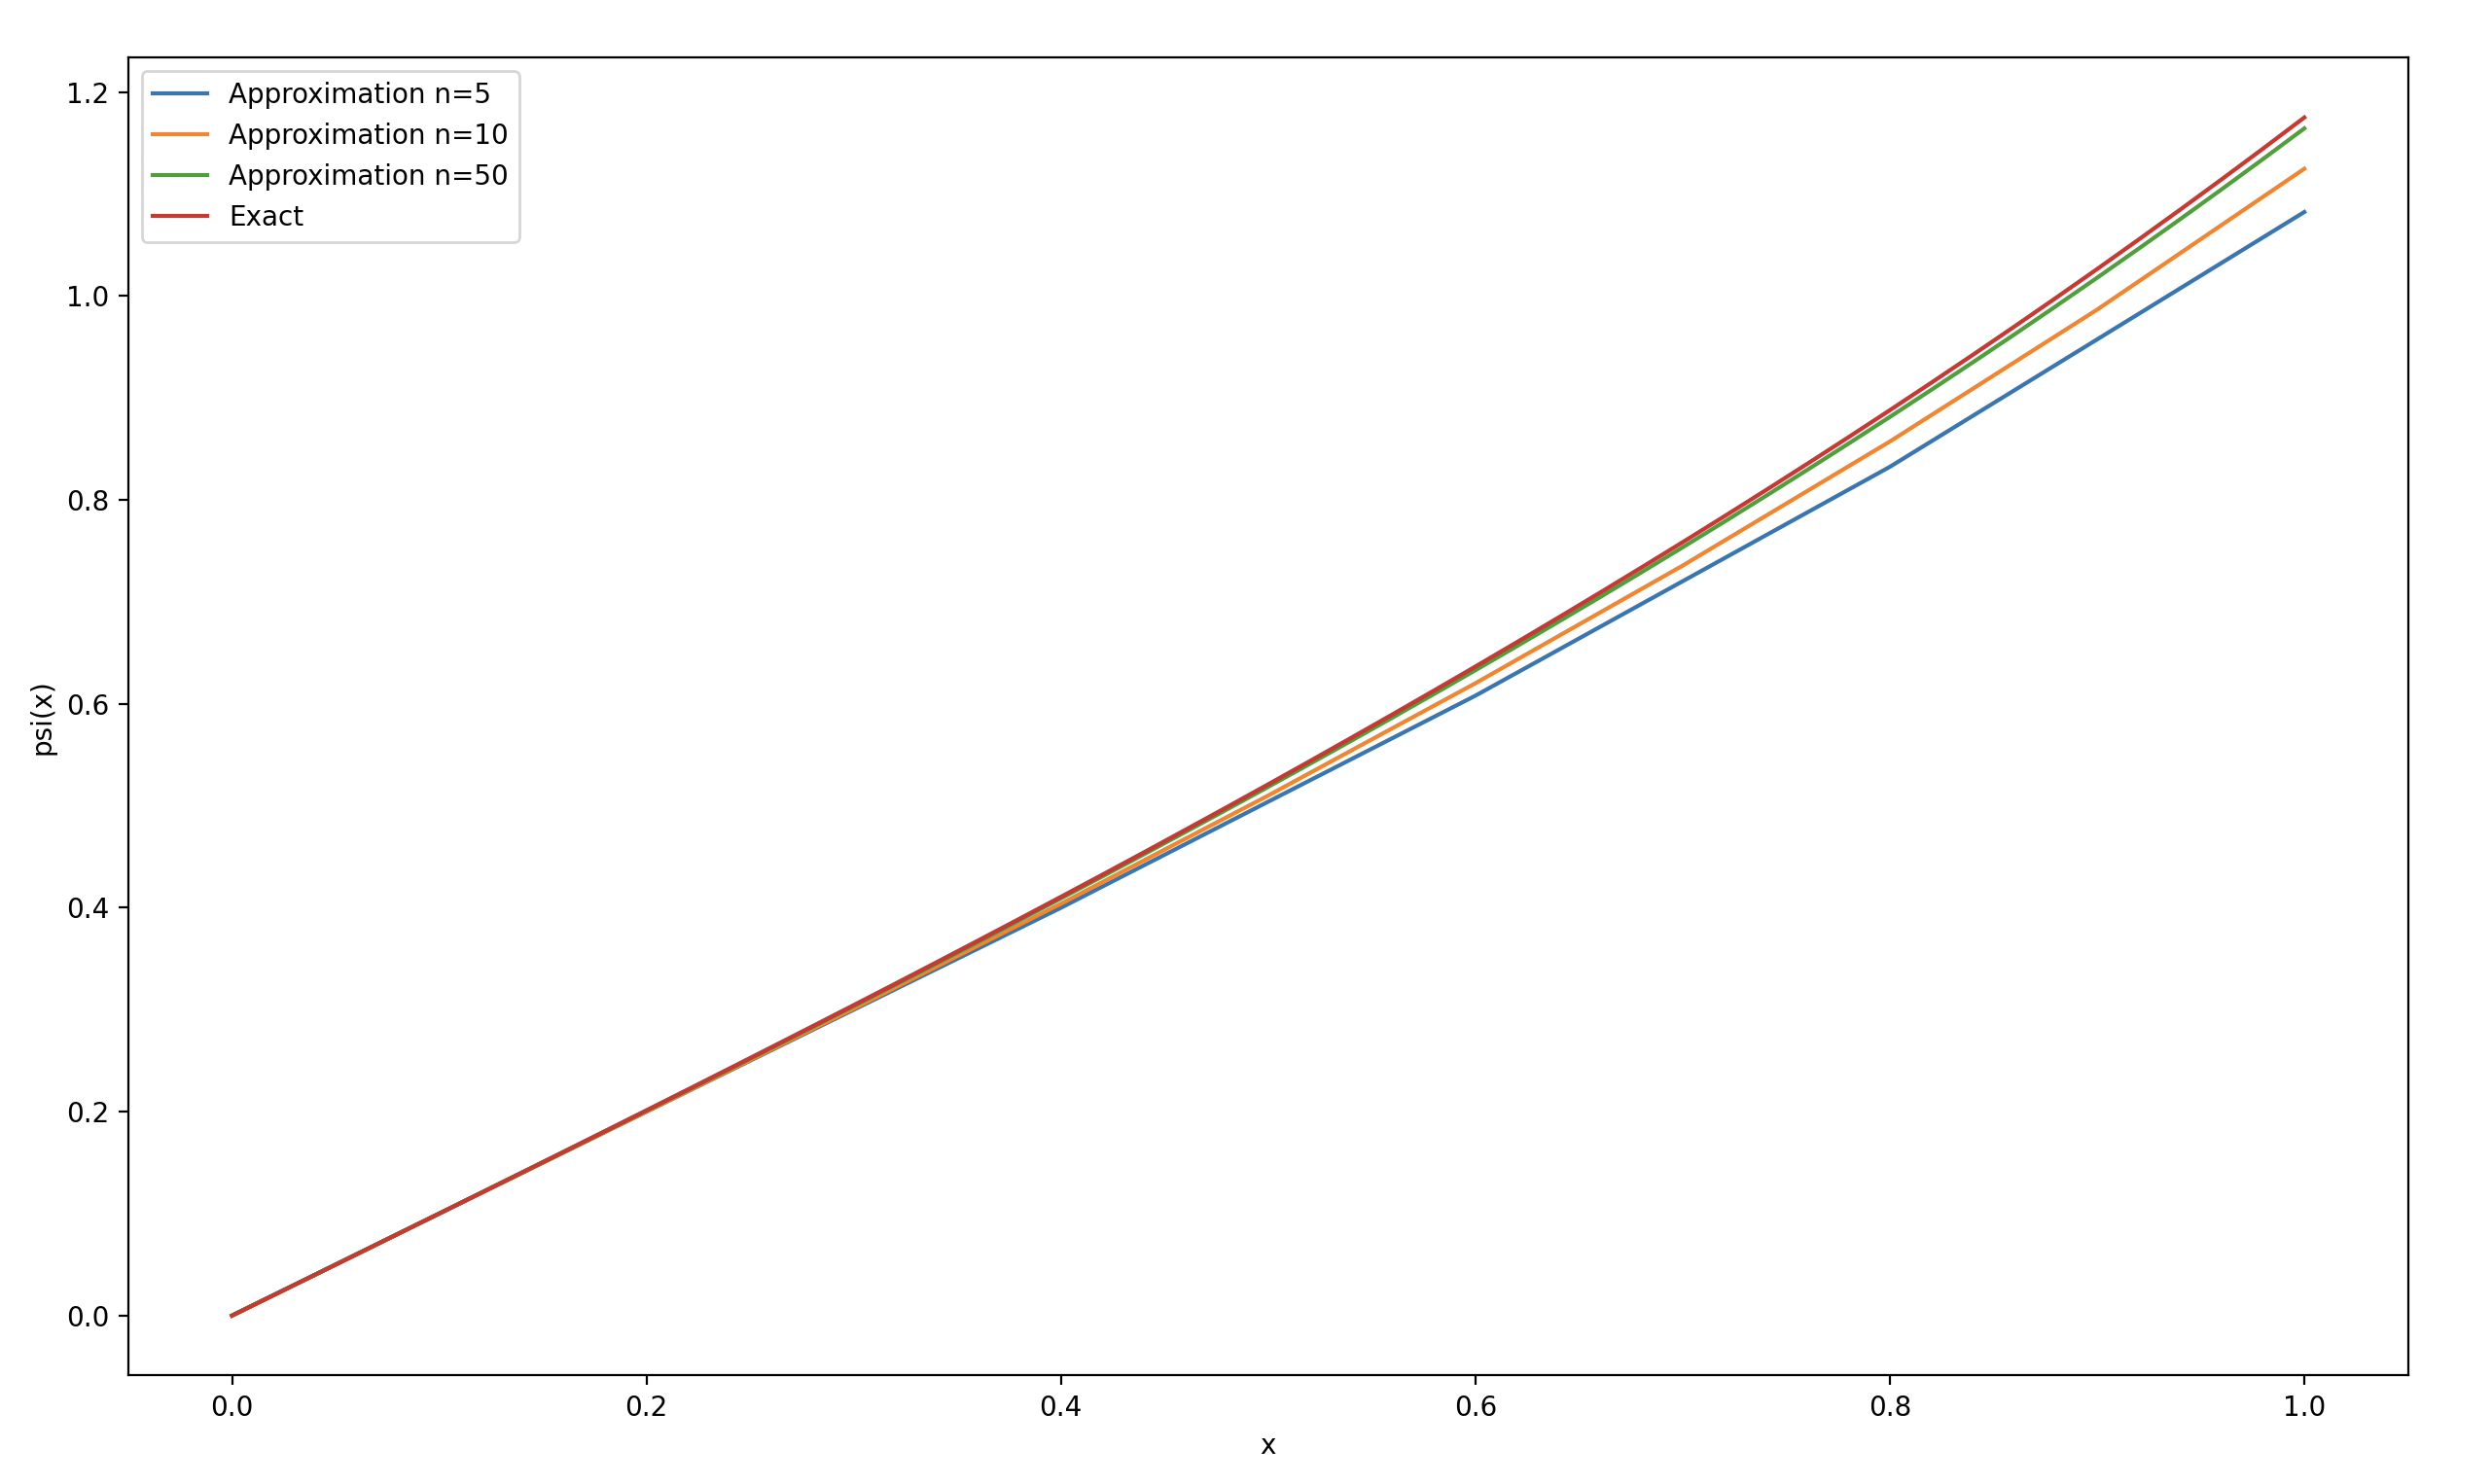
\includegraphics[scale=0.215]{ch7-7.65.png}
\end{center} 
\end{proof}

\cleardoublepage
\begin{proof}{\textbf{7.66}}
All plots were generated using the file \verb|ch7-7.66.py|.
\begin{itemize}
    \item [\textbf{(a)}] The Gaussian well of Problem 7.37 looks like the
    following
    \begin{center}
        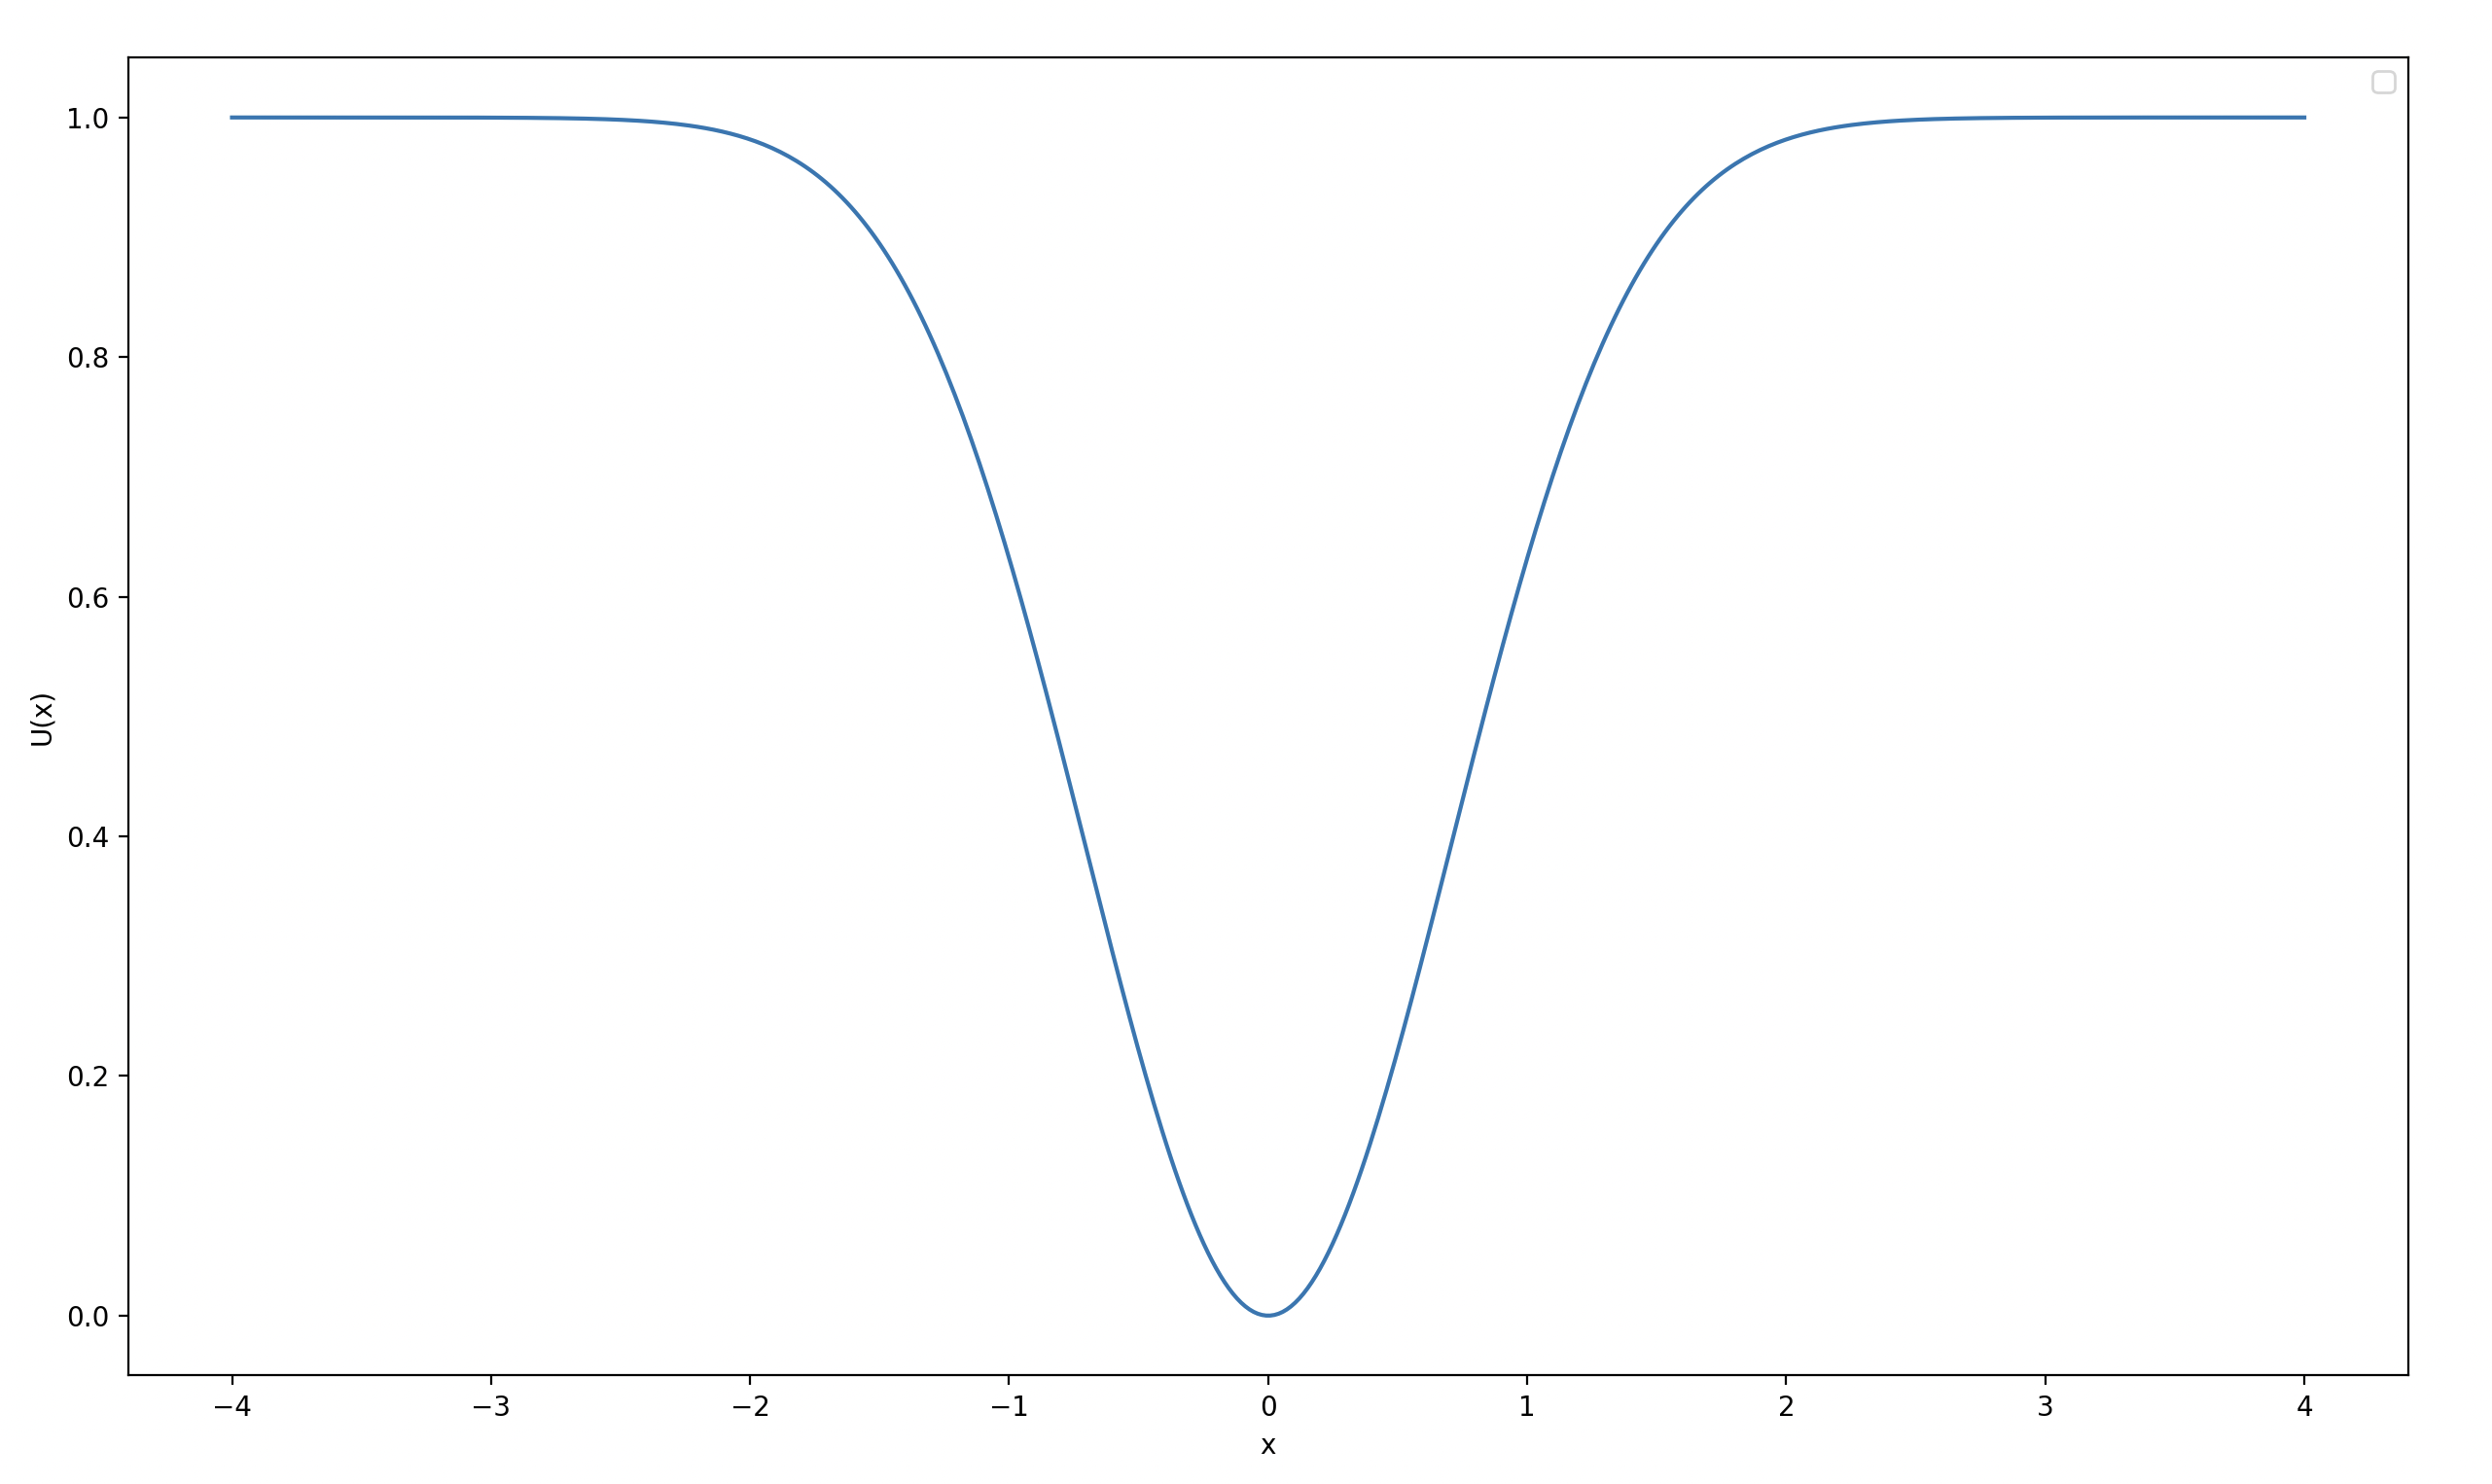
\includegraphics[scale=0.25]{ch7-7.66-i.png}
    \end{center}
    \item [\textbf{(b)}] Solving Schrödinger equation using the Runge-kutta
    method for $E = 0.1$ we get that
    \begin{center}
        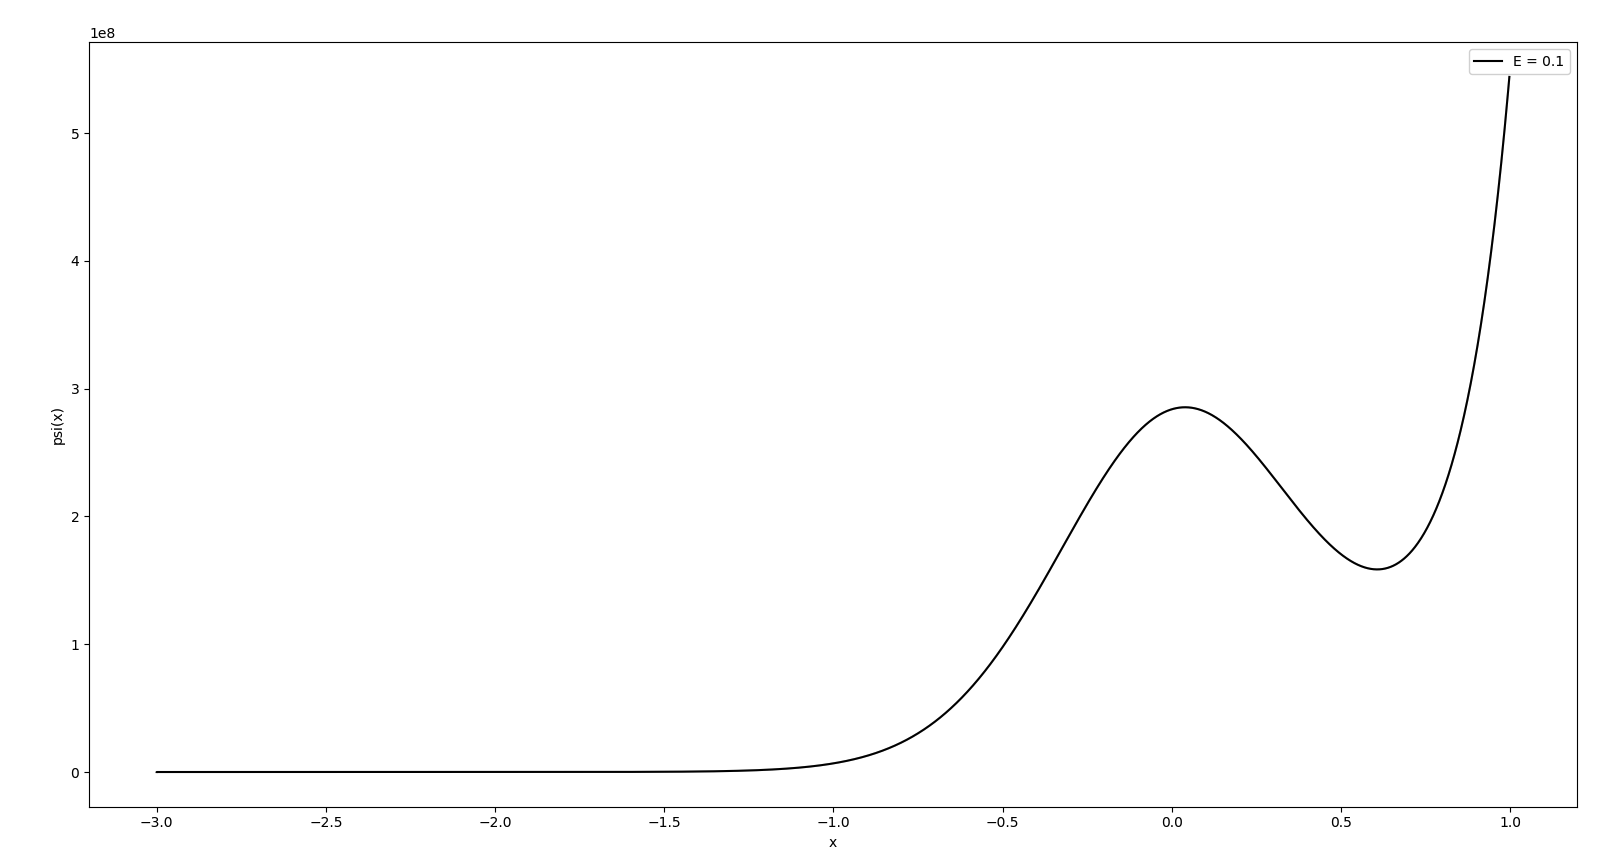
\includegraphics[scale=0.22]{ch7-7.66-ii.png}
    \end{center}

\cleardoublepage
    \item [\textbf{(c)}] Solving Schrödinger equation using the Runge-kutta
    method for $E = 0.2$ we get that
    \begin{center}
        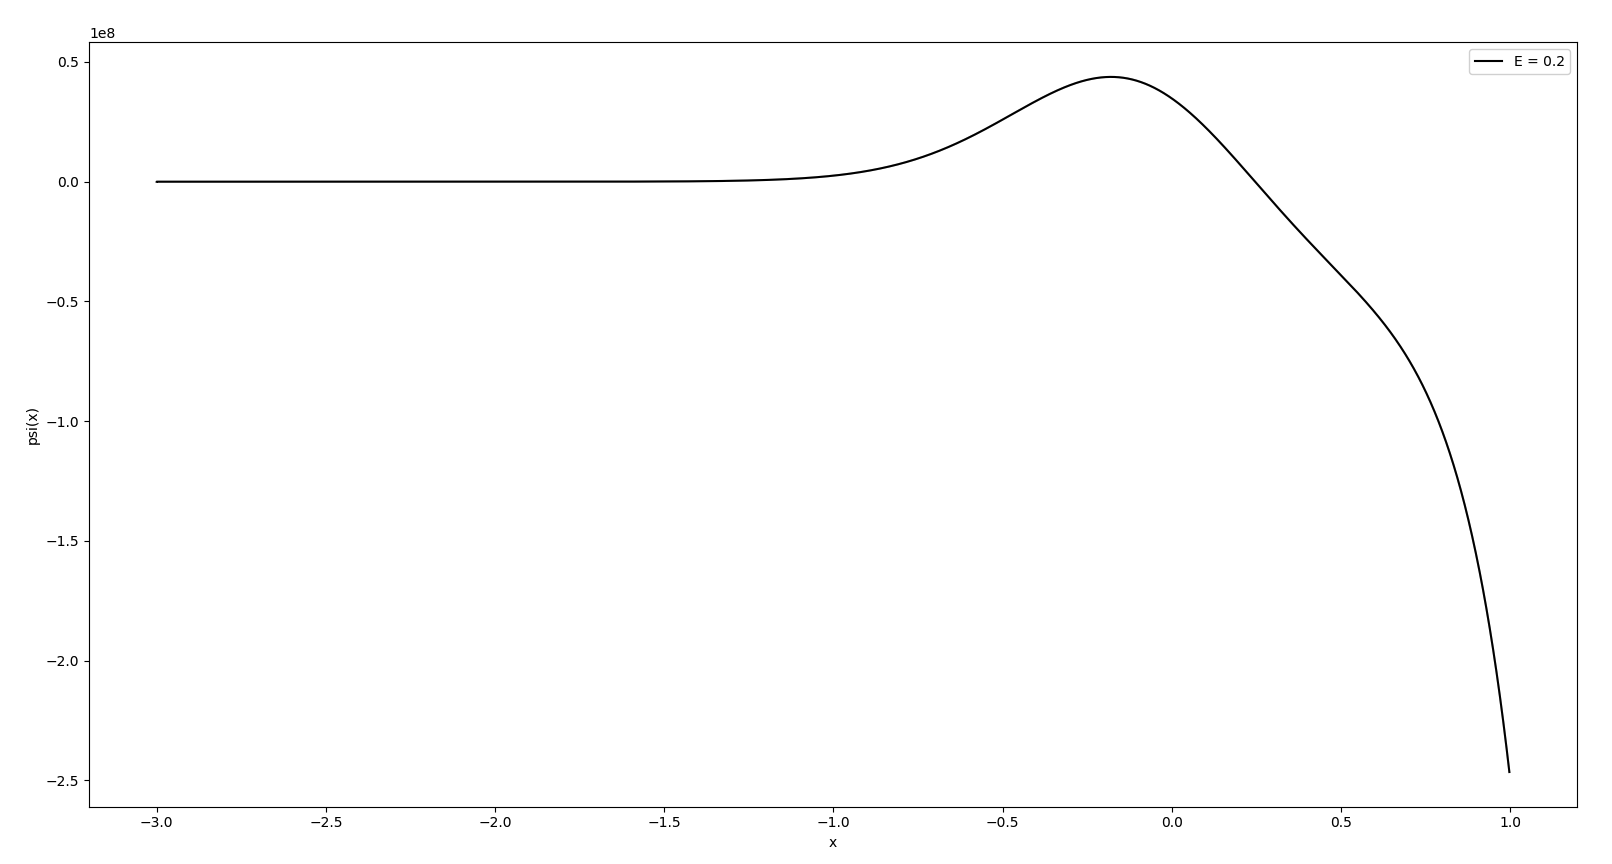
\includegraphics[scale=0.22]{ch7-7.66-iii.png}
    \end{center}
    From part (b) and (c) we can conclude that the ground-state energy must be
    between $E = 0.1$ and $E = 0.2$.
    \item [\textbf{(d)}] We plot a few solutions of the Schrödinger equation
    for different energies to get the ground-state energy
    \begin{center}
        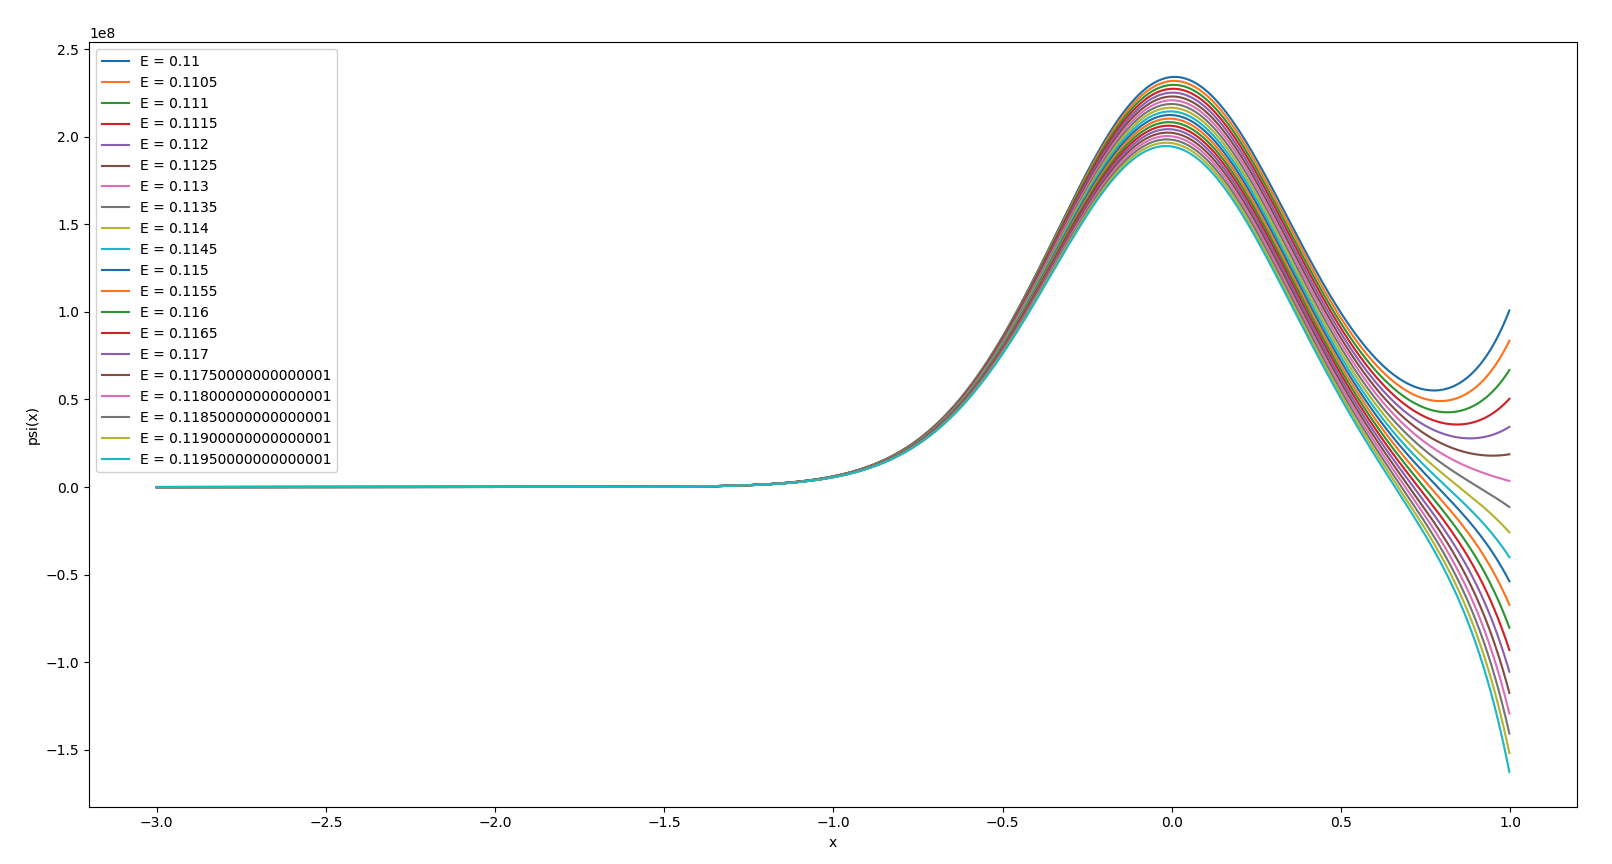
\includegraphics[scale=0.22]{ch7-7.66-iv.png}
    \end{center}
    We see that the energy value for which the solution doesn't diverge is
    approximately $E = 0.113$, and hence this is an approximated value for
    the ground-state energy.

\end{itemize}
\end{proof}

\cleardoublepage
\begin{proof}{\textbf{7.67}}
\begin{itemize}
\item [\textbf{(a)}] We know that the symmetric solution within the well is 
\begin{align*}
    \psi(x) = G\cos(kx)
\end{align*}
And outside the well for $x < -a/2$ must be
\begin{align*}
    \psi(x) = Ae^{\alpha x}
\end{align*}
Bus since $\psi(x)$ is continuous at $x = -a/2$ must happen that
\begin{align*}
    Ae^{-\alpha a/2} = G\cos(ka/2)
\end{align*}
On the other hand, $\psi'(x)$ is also continuous at $x = -a/2$ hence we get
that
\begin{align*}
    \alpha Ae^{-\alpha a/2} = kG\sin(ka/2)
\end{align*}
Finally, dividing both equations we get that
\begin{align*}
    \frac{\alpha e^{-\alpha a/2}}{e^{-\alpha a/2}}
    &= \frac{k\sin(ka/2)}{\cos(ka/2)}\\
    \alpha &= k \tan(ka/2)
\end{align*}

\item [\textbf{(b)}] We know that
\begin{align*}
    \alpha &= \frac{\sqrt{2m(U_0 - E)}}{\hbar}
    \quad\text{and}\quad
    k = \frac{\sqrt{2mE}}{\hbar}
\end{align*}
Replacing the value of $\alpha$ on the equation we determined on part
\textbf{(a)} we get that
\begin{align*}
    \frac{\sqrt{2m(U_0 - E)}}{\hbar} &= k \tan(ka/2)\\
    \atan(\frac{\sqrt{2m(U_0 - E)}}{k\hbar}) &= \frac{ka}{2}
\end{align*}
Then if we let $U_0 \to \infty$ and we replace $k$ we have that
\begin{align*}
    \frac{a\sqrt{2mE}}{2\hbar} &= \frac{\pi}{2}\\
    \sqrt{2mE} &= \frac{\pi\hbar}{a}\\
    E &= \frac{\pi^2\hbar^2}{2ma^2}
\end{align*}
Which is the correct ground state energy for the case of a rigid box
($U_0 \to \infty$).

\cleardoublepage
\item [\textbf{(c)}]
Replacing $\alpha$, $k$ and $U_0 = 3E_1$ we get that
\begin{align*}
    \frac{\sqrt{4mE_1}}{\hbar}
    &= \frac{\sqrt{2mE_1}}{\hbar}\tan(\frac{a\sqrt{2mE_1}}{2\hbar})\\
    4mE_1 &= 2mE_1\tan[2](\frac{a\sqrt{2mE_1}}{2\hbar})\\
    \atan(\sqrt{2}) &= \frac{a\sqrt{2mE_1}}{2\hbar}\\
    \frac{4\hbar^2}{a^2}\atan[2](\sqrt{2}) &= 2mE_1
\end{align*}
Hence
\begin{align*}
    E_1 &= \frac{2\hbar^2}{ma^2}\atan[2](\sqrt{2})
    = \frac{2.03\sci{-68}~kg^2m^4/s^2}{ma^2}
\end{align*}

\end{itemize}
\end{proof}

\end{document}